%%%%%%%%%%%%%%%%%%%%%%%%%%%%%%%%%%%
% PART I: User's manual
%%%%%%%%%%%%%%%%%%%%%%%%%%%%%%%%%%%

\part{User's manual}
\label{part:1}

\chapter{A \GLOBES\ tour}
\label{chapter:tour}
\index{GLoBES tour}

In this first chapter, we show a \GLOBES\ tour illustrating the
main features of \GLOBES . The complete example  
can be found as {\tt example-tour.c} in the example subdirectory of your \GLOBES\ distribution.
The output is written to {\tt stream}, which can be either {\tt stdout},
or a file. Details about how to use \GLOBES\ with C can found in \Chapt~\ref{chapt:gettingstarted} and the following chapters.
You can also find a summary of the most important \GLOBES\ $\chi^2$-functions in \tabl{stdfunctions}. Note that this chapter
can be skipped without loss of relevant information.

\begin{table}[tpb]
\begin{center}
\begin{tabular}{p{3.8cm}p{3.8cm}p{7cm}}
\hline
Function & Purpose & Parameters \ra\ Result \\
\hline
\multicolumn{3}{l}{{\bf Systematics only:}} \\
\GLB{glbChiSys} & $\chi^2$ with systematics only  & ({\tt glb\_params in, int exp, int rule}) \ra\  {\tt double} $\chi^2$ \\[0.2cm]
\multicolumn{3}{l}{{\bf Projections onto axes:}} \\
\GLB{glbChiTheta} & Projection onto $\theta_{13}$-axis  &  ({\tt glb\_params in, glb\_params out, int exp}) \ra\  {\tt double} $\chi^2$ \\[0.1cm]
\GLB{glbChiDelta} & Projection onto $\deltacp$-axis  &  ({\tt glb\_params in, glb\_params out, int exp}) \ra\  {\tt double} $\chi^2$ \\[0.1cm]
\GLB{glbChiTheta23} & Projection onto $\theta_{23}$-axis  &  ({\tt glb\_params in, glb\_params out, int exp}) \ra\  {\tt double} $\chi^2$ \\[0.1cm]
\GLB{glbChiDm} & Projection onto $\ldm$-axis  &  ({\tt glb\_params in, glb\_params out, int exp}) \ra\  {\tt double} $\chi^2$ \\[0.1cm]
\GLB{glbChiDms} & Projection onto $\sdm$-axis  &  ({\tt glb\_params in, glb\_params out, int exp}) \ra\  {\tt double} $\chi^2$ \\[0.2cm]
\multicolumn{3}{l}{{\bf Projection onto plane:}} \\
\GLB{glbChiThetaDelta} & Projection onto $\theta_{13}$-$\deltacp$-plane  &  ({\tt glb\_params in, glb\_params out, int exp}) \ra\  {\tt double} $\chi^2$ \\[0.2cm]
\multicolumn{3}{l}{{\bf Projection onto any hyper-plane:}} \\
\GLB{glbChiNP} & Projection onto any $n$-dimensional hyper-plane  &  ({\tt glb\_params in, glb\_params out, int exp}) \ra\  {\tt double} $\chi^2$ \newline
Needs \GLB{glbSetProjection} before! \\[0.2cm]
\multicolumn{3}{l}{{\bf Localization of degeneracies:}} \\
\GLB{glbChiAll} & (Local) Minimization over all parameters  &  ({\tt glb\_params in, glb\_params out, int exp}) \ra\  {\tt double} $\chi^2$ \\
\hline
\end{tabular}
\end{center}
\caption{\label{tab:stdfunctions} \index{Standard functions (table)} The \GLOBES\ standard function to obtain a $\chi^2$-value with systematics only or systematics and correlations. The parameters {\tt rule} and {\tt exp}
can either be \GLB{GLB\_ALL} for all initialized experiment or the
experiment number ($0$ to \GLB{glb\_num\_of\_exps}-1) for a specific experiment. The format of \GLB{glb\_params} is discussed in detail in \Chapt~\ref{chapt:gettingstarted}. Note that all functions but {\tt ChiSys}
  are using minimizers which have to be initialized with \GLB{glbSetInputErrors} and \GLB{glbSetStartingValues} first.}
\end{table}

\vspace*{0.5cm}

\noindent Initialize the \GLOBES\ library:
\gq{
glbInit(argv[0]);
} 
Define my standard oscillation parameters:
\gq{
double theta12 = asin(sqrt(0.8))/2; \\
double theta13 = asin(sqrt(0.001))/2;\\
double theta23 = M\_PI/4;\\
double deltacp = M\_PI/2;\\
double sdm = 7e-5;\\
double ldm = 2e-3;
}
Load one neutrino factory experiment:
\gq{
glbInitExperiment("NuFact.glb",\&glb\_experiment\_list[0], \\ \hspace*{4cm} \&glb\_num\_of\_exps);
} 
Initialize a number of parameter vectors we are going to use later:
\gq{
glb\_params true\_values = glbAllocParams();\\
glb\_params fit\_values = glbAllocParams();\\
glb\_params starting\_values = glbAllocParams();\\
glb\_params input\_errors = glbAllocParams();\\
glb\_params minimum = glbAllocParams();
}
Assign values to our standard oscillation parameters:
\gq{
 glbDefineParams(true\_values,theta12,theta13,theta23,deltacp,sdm,ldm);
}
Compute the simulated data with our standard parameters:
\gq{
 glbSetOscillationParameters(true\_values); \\
 glbSetRates();
}
Return the oscillation probabilities in vacuum and matter for the
electron neutrino as initial flavor:
\gq{
 int i; \\
 fprintf(stream,"$\backslash$nOscillation probabilities in vacuum: ");\\
 for(i=1;i<4;i++) fprintf(stream,"1->\%i: \%g",i, \\
 \hspace*{4cm} glbVacuumProbability(1,i,+1,50,3000)); \\ 
 fprintf(stream,"$\backslash$nOscillation probabilities in matter: ");\\
 for(i=1;i<4;i++) fprintf(stream,"1->\%i: \%g ",i,\\ \hspace*{4cm} glbProfileProbability(1,i,+1,50)); \\
}
\go{
Oscillation probabilities in vacuum: 1->1: 0.999953 1->2: 2.69441e-05 1->3: 1.98019e-05 \\
Oscillation probabilities in matter: 1->1: 0.999965 1->2: 2.02573e-05 1->3: 1.49021e-05 
}
Now assign fit values, where we will test the fit value $\stheta=0.0015$:
\gq{
 glbCopyParams(true\_values,fit\_values); \\
 glbSetOscParams(fit\_values,asin(sqrt(0.0015))/2,GLB\_THETA\_13);
}
Compute $\chi^2$ with systematics only for all experiments and rules:
\gq{
  chi2 = glbChiSys(fit\_values,GLB\_ALL,GLB\_ALL); \\
  fprintf(stream,"chi2 with systematics only: \%g$\backslash$n$\backslash$n",chi2);
}
\go{
chi2 with systematics only: 22.3984
}
This we would obtain from the first appearance channel only:
\gq{
 chi2 = glbChiSys(fit\_values,0,0);\\
 fprintf(stream,"This we would have from the CP-even appearance channel only: \%g$\backslash$n$\backslash$n",chi2);
}
\go{
This we would have from the CP-even appearance channel only: 21.6223
}
The sum over all rules again gives:
\gq{
 chi2 = glbChiSys(fit\_values,GLB\_ALL,0)+ 
        glbChiSys(fit\_values,GLB\_ALL,1)+ \\  
\hspace*{1.3cm} glbChiSys(fit\_values,GLB\_ALL,2)+          glbChiSys(fit\_values,GLB\_ALL,3); \\ 
\mbox{fprintf(stream,"The sum over all rules gives again: \%g$\backslash$n$\backslash$n",chi2);}
}
\go{
The sum over all rules gives again: 22.3984
}
Let's prepare the minimizers for taking into account correlations.
Set errors for external parameters, too: 10\% for each of the solar parameters, and 5\% for the matter density. 
\gq{
 glbDefineParams(input\_errors,theta12*0.1,0,0,0,sdm*0.1,0); \\
 glbSetDensityParams(input\_errors,0.05,GLB\_ALL); \\
 glbSetStartingValues(true\_values); \\
 glbSetInputErrors(input\_errors);
}
Then we can calculate $\chi^2$ including the full multi-parameter
correlation, and show where \GLOBES\ actually found the minimum
(note that this takes somewhat longer than systematics only). 
This corresponds to a projection onto the $\stheta$-axis:
\gq{
 chi2 = glbChiTheta(fit\_values,minimum,GLB\_ALL); \\ 
 fprintf(stream,"chi2 with correlations: \%g $\backslash$n",chi2); \\
 fprintf(stream,"Position of minimum: theta12, theta13, theta23, \\ \hspace*{0.5cm} delta, sdm, ldm, rho$\backslash$n"); \\
 glbPrintParams(stream,minimum); \\ 
 fprintf(stream,"Note that s22theta13 is unchanged/kept fixed: \\
 \hspace*{0.5cm} \%g! $\backslash$n$\backslash$n",    pow(sin(2*glbGetOscParams(minimum,GLB\_THETA\_13)),2));
}
\go{
chi2 with correlations: 2.1038 \\
Position of minimum: theta12,theta13,theta23,delta,sdm,ldm,rho \\
0.542002 0.0193698 0.747915 1.77688 6.66156e-05 0.00200817 \\
1.00434 \\
Iterations: 1693 \\
Note that s22theta13 is unchanged/kept fixed: 0.0015! 
}
Instead of including the full correlation, we can take the
correlation with every parameter except from $\deltacp$, \ie,
we keep (in addition to $\theta_{13}$) $\deltacp$ fixed.
This corresponds to projection onto the $\stheta$-$\deltacp$-plane:
\gq{
 chi2 = glbChiThetaDelta(fit\_values,minimum,GLB\_ALL); \\
fprintf(stream,"chi2 with correlations other than with deltacp: \%g $\backslash$n$\backslash$n",chi2); 
}
\go{
chi2 with correlations other than with deltacp: 4.32831 
}
Similarly, we can only take into account the correlation with $\deltacp$.
For this, we need to define our own (user-defined) projection, where
only $\deltacp$ is a free parameter:
\gq{
 glb\_projection myprojection = glbAllocProjection(); \\
 glbDefineProjection(myprojection,GLB\_FIXED, GLB\_FIXED, GLB\_FIXED, \\
 \hspace*{0.5cm} GLB\_FREE, GLB\_FIXED, GLB\_FIXED); \\
 glbSetProjection(myprojection); \\
 chi2 = glbChiNP(fit\_values,minimum,GLB\_ALL); \\
 fprintf(stream,"chi2 with correlation only with deltacp: \\
 \hspace*{0.5cm} \%g $\backslash$n$\backslash$n",chi2); \\
 glbFreeProjection(myprojection); 
}  
\go{
chi2 with correlation only with deltacp: 2.80651 
}
We can also switch of the systematics and compute the
statistics $\chi^2$ only:
\gq{
 glbSwitchSystematics(GLB\_ALL,GLB\_ALL,GLB\_OFF); \\   
 chi2 = glbChiSys(fit\_values,GLB\_ALL,GLB\_ALL); \\
 glbSwitchSystematics(GLB\_ALL,GLB\_ALL,GLB\_ON); \\   
 fprintf(stream,"chi2 with statistics only: \\ 
 \hspace*{0.5cm} \%g$\backslash$n$\backslash$n",chi2);
}
\go{
chi2 with statistics only: 39.143
}
Let us now locate the exact position of the sgn-degeneracy:
\gq{
  glbDefineParams(input\_errors,theta12*0.1,0,0,0,sdm*0.1,ldm/3); \\
  glbDefineParams(starting\_values,theta12,theta13,theta23, \\
  \hspace*{0.5cm} deltacp,sdm,-ldm); \\
  glbSetDensityParams(input\_errors,0.05,GLB\_ALL); \\
  glbSetStartingValues(starting\_values);\\
  glbSetInputErrors(input\_errors);\\
  chi2=glbChiAll(starting\_values,minimum,GLB\_ALL);\\ 
  fprintf(stream,"chi2 at minimum: \%g $\backslash$n",chi2);\\
  fprintf(stream,"Position of minimum: \\ \hspace*{0.5cm} theta12,theta13,theta23,delta,sdm,ldm,rho$\backslash$n"); \\
  glbPrintParams(stream,minimum); 
}
\go{
chi2 at minimum: 6.20025 \\
Position of minimum: theta12,theta13,theta23,delta,sdm,ldm,rho \\
0.591812 0.0264717 0.72763 1.08709 8.0004e-05 -0.00206094 \\
0.970685  \\
Iterations: 1946 \\
}
After testing these functions with only one experiment, let us now
go to a two-experiment setup with two different neutrino factory baselines.
Since the \GLOBES\ parameter vectors depend on the number of experiments,
we have to destroy them first:
\gq{
 glbFreeParams(true\_values); \\
 glbFreeParams(fit\_values); \\ 
 glbFreeParams(starting\_values);\\
 glbFreeParams(input\_errors);\\
 glbFreeParams(minimum);
}
Then we clear the experiment list and load the new experiments:
\gq{
 fprintf(stream,"$\backslash$nNOW: TWO-EXPERIMENT SETUP \\
 \hspace*{0.5cm} NuFact at 3000km+NuFact at 7500km$\backslash$n$\backslash$n"); \\
 \\
  glbClearExperimentList(); \\
\\
 glbInitExperiment("NuFact.glb",\&glb\_experiment\_list[0], \\
 \hspace*{0.5cm} \&glb\_num\_of\_exps);\\
  glbInitExperiment("NuFact.glb",\&glb\_experiment\_list[0], \\
 \hspace*{0.5cm} \&glb\_num\_of\_exps);
}
\go{
NOW: TWO-EXPERIMENT SETUP NuFact at 3000km+NuFact at 7500km
}
Then we need to change the baseline of the second experiment, where
we set the density to the average density of this baseline:
\gq{
  double* lengths;  \\
  double* densities; \\
 glbAverageDensityProfile(7500,\&lengths,\&densities);\\
  fprintf(stream,"Magic baseline length: \%g, \\
  \hspace*{0.5cm} Density: \%g$\backslash$n$\backslash$n",lengths[0],densities[0]); \\
 glbSetProfileDataInExperiment(1,1,lengths,densities); \\
   free(lengths); \\
   free(densities);
}
\go{
 Magic baseline length: 7500, Density: 4.25286
}
Now we can re-initialize our parameter vectors again:
\gq{
 true\_values = glbAllocParams();\\
 fit\_values = glbAllocParams(); \\
 starting\_values = glbAllocParams(); \\
 input\_errors = glbAllocParams(); \\
 minimum = glbAllocParams(); \\
 glb\_params minimum2 = glbAllocParams(); 
}
In addition, we repeat the procedure for the simulated rates and
the fit parameter vector:
\gq{
  glbDefineParams(true\_values,theta12,theta13,theta23,deltacp,sdm,ldm); \\
  glbSetOscillationParameters(true\_values); \\
  glbSetRates();\\
  \\
  glbCopyParams(true\_values,fit\_values);\\
  glbSetOscParams(fit\_values,asin(sqrt(0.0015))/2,GLB\_THETA\_13);
} 
Here comes the $\chi^2$ with systematics only for all experiments and
rules:
\gq{
 chi2 = glbChiSys(fit\_values,GLB\_ALL,GLB\_ALL); \\
 fprintf(stream,"chi2 with systematics for all exps: \\ 
 \hspace*{0.5cm} \%g$\backslash$n",chi2); 
}
\go{
 chi2 with systematics for all exps: 31.0797
}
Compute $\chi^2$ for each experiment and compute the sum:
\gq{
  chi2 = glbChiSys(fit\_values,0,GLB\_ALL); \\
 fprintf(stream,"chi2 with systematics for 3000km: \%g$\backslash$n",chi2); \\
 chi2b = glbChiSys(fit\_values,1,GLB\_ALL); \\
 fprintf(stream,"chi2 with systematics for 7500km: \%g$\backslash$n",chi2b);
 \\
  fprintf(stream,"The two add again to: \newline
  \hspace*{0.5cm} \%g$\backslash$n$\backslash$n",chi2+chi2b);
}
\go{
chi2 with systematics for 3000km: 22.3984 \\
chi2 with systematics for 7500km: 8.68131 \\
The two add again to: 31.0797
}
Similarly, compute the $\chi^2$ with correlations for each experiment
and their combination. Compare it to the $\chi^2$ for all experiments:
the sum of the individual results is not equal to the $\chi^2$ of the
combination anymore. Note that there are now two densities in the
output vectors. 
\gq{
 glbDefineParams(input\_errors,theta12*0.1,0,0,0,sdm*0.1,0); \\
 glbSetDensityParams(input\_errors,0.05,GLB\_ALL); \\
 glbSetStartingValues(true\_values); \\
 glbSetInputErrors(input\_errors); \\
 chi2 = glbChiTheta(fit\_values,minimum,0);\\ 
  fprintf(stream,"chi2 with correlations for 3000km: \%g $\backslash$n",chi2); \\
 glbPrintParams(stream,minimum); \\ 
  chi2b = glbChiTheta(fit\_values,minimum,1); \\ 
 fprintf(stream,"$\backslash$nchi2 with correlations for 7500km: \\
  \hspace*{0.5cm}  \%g $\backslash$n",chi2b); \\
  glbPrintParams(stream,minimum); \\ 
 chi2sum = glbChiTheta(fit\_values,minimum,GLB\_ALL); \\ 
 fprintf(stream,"$\backslash$nchi2 with correlations for combination: \\
  \hspace*{0.5cm} \%g $\backslash$n",chi2sum); \\
 glbPrintParams(stream,minimum); \\ 
  fprintf(stream,"$\backslash$nThe sum of the two chi2s is \%g,  \\
  \hspace*{0.5cm} whereas the total chi2 is \%g !$\backslash$n$\backslash$n",chi2+chi2b,chi2sum); 
}
\go{
chi2 with correlations for 3000km: 2.1038 \\
0.542002 0.0193698 0.747915 1.77688 6.66156e-05 0.00200817 \\ 
1.00434 1 \\
Iterations: 1693 \\
\\
chi2 with correlations for 7500km: 1.08421 \\
0.557356 0.0193698 0.771359 4.77751 7.00762e-05 0.00200105 \\
1 1.01517 \\
Iterations: 661 \\
\\
chi2 with correlations for combination: 3.90835  \\
0.544432 0.0193698 0.770175 1.78502 6.61621e-05 0.00200303 \\ 
1.00431 1.03679 \\
Iterations: 1636 \\
\\
The sum of the two chi2s is 3.18801, whereas the total chi2 is 3.90835!
}
Now find the $\mathrm{sgn}(\ldm)$-degeneracies for both individual
experiments and test if they are still there in the combination of the
experiments. Note that a minimum at a negative value of $\theta_{13}$ is unphysical. However, if there can be no degeneracy found at a positive value, there is probably none at a low confidence level.  
\gq{
 glbDefineParams(input\_errors,theta12*0.1,theta13,theta23, \\
 \hspace*{0.5cm} deltacp,sdm*0.1,ldm/3); \\
glbDefineParams(starting\_values,theta12,theta13,theta23, \\
\hspace*{0.5cm} deltacp,sdm,-ldm);\\
  glbSetDensityParams(input\_errors,0.05,GLB\_ALL);\\
  glbSetStartingValues(starting\_values);\\
  glbSetInputErrors(input\_errors);\\
  \\
  chi2=glbChiAll(starting\_values,minimum,0); \\ 
  fprintf(stream,"chi2 at minimum, L=3000km: \%g $\backslash$n",chi2); \\
  glbPrintParams(stream,minimum);   \\
  \\
  chi2b=glbChiAll(starting\_values,minimum2,1);  \\
  \mbox{fprintf(stream,"$\backslash$nchi2 at minimum, L=7500km: \%g \\ $\backslash$n",chi2b);} \\
  glbPrintParams(stream,minimum2);  \\
  \\
  chi2=glbChiAll(minimum,minimum,GLB\_ALL); \\
  fprintf(stream,"$\backslash$nchi2 for combination at minimum of Exp. 1:\\ \hspace*{0.5cm} \%g $\backslash$n",chi2); \\
  glbPrintParams(stream,minimum);  \\
  \\
  chi2b=glbChiAll(minimum2,minimum2,GLB\_ALL); \\
  fprintf(stream,"$\backslash$nchi2 for combination at minimum of Exp. 2: \\
  \hspace*{0.5cm} \%g $\backslash$n",chi2b); \\
  glbPrintParams(stream,minimum2);  
}
\go{
chi2 at minimum, L=3000km: 6.71794 \\
0.591497 0.0257396 0.729058 1.11537 7.98867e-05 -0.00206005 \\
0.970499 1 \\
Iterations: 2104\\
\\
chi2 at minimum, L=7500km: 47.1013 \\
0.590347 0.0018489 0.768372 0.984827 8.23415e-05 -0.00204588 \\
1 0.780995 \\
Iterations: 1270\\
\\
chi2 for combination at minimum of Exp. 1: 70.6353 \\
0.607988 0.0165985 0.767682 1.41422 8.44573e-05 -0.00204853 \\
0.96147 1.1831 \\
Iterations: 1549 \\
\\
chi2 for combination at minimum of Exp. 2: 70.6357 \\
0.608454 0.0165823 0.767757 1.41481 8.43864e-05 -0.00204853 \\
0.961129 1.18304 \\
Iterations: 1447 
}
Finally, we have to destroy the parameter vectors again:
\gq{
 glbFreeParams(true\_values); \\
 glbFreeParams(fit\_values); \\
 glbFreeParams(starting\_values); \\
 glbFreeParams(input\_errors); \\
 glbFreeParams(minimum); \\
 glbFreeParams(minimum2); \\
}

\chapter{\GLOBES\ basics}
\label{chapt:gettingstarted}

\index{Installation}
In this first chapter of the user's manual, we assume that the \GLOBES\ software is readily installed on your computer system. For the installation,
see \App~\ref{app:installation} and the {\tt INSTALL} file in the
software package. We demonstrate how to load pre-defined experiments 
and introduce the basic concepts of \GLOBES . We do not go
into details of the programming language, which means that standard parts
of the program code common to all of the examples in the following chapters are, in general, omitted.
An example of a minimal \GLOBES\ program in C can be found on page~\pageref{ex:c}. Furthermore, the files of the examples in this part can be found in the {\tt Example} subdirectory of your \GLOBES\ distribution. \index{Examples} Since it depends on your installed
configuration, we refer to the {\tt README} file in the \GLOBES\ main directory, and the comments in the Makefile of the {\tt Example} subdirectory for how to compile the example files. Make sure that
the data files (\AEDL\ and supporting files) in the {\tt data} 
subdirectory can be found by the
examples. In case of doubt, you can simply copy the necessary files
into the working directory where the examples are executed.

We will in this part not go into details of the experiment
definition. The pre-defined experiment prototypes in the {\tt data}
subdirectory are summarized in \tabl{experiments}. They correspond
(except from minor modifications) to the experiments in the
respective references in the table.

\example{Using \GLOBES\ with C}{\label{ex:c}
\index{C-Code}
\index{Program}
Here comes the C-code skeleton, which is
(more or less) common to all of our \GLOBES\ examples:
\begin{quote}
{\tt {\footnotesize
\#include <stdio.h> \\
\#include <stdlib.h> \\
\#include <math.h> \\
\#include <string.h> \\
\\
\#include <globes/globes.h> \hspace*{0.5cm} /* Include GLoBES library */ \\
\\
\#include "myio.h" \hspace*{0.5cm} /* Include "housemade" I/O-routines */ \\
\\
/* If filename given, write to file; if empty, to screen: */ \\
char MYFILE[]="testX.dat"; \\
\\
int main(int argc, char *argv[]) \\
\{  \\
\\
 \hspace*{0.5cm} glbInit(argv[0]); \hspace*{0.5cm} /* Initialize GLoBES library */ \\
\\  
  \hspace*{0.5cm} glbInitExperiment("NuFact.glb",\&glb\_experiment\_list[0], \\
  \hspace*{1cm} \&glb\_num\_of\_exps); \hspace*{0.5cm} /* Initialize experiment NuFact.glb */\\
\\  
  \hspace*{0.5cm}  /* Initialize housemade output function */\\
  \hspace*{0.5cm} 
   InitOutput(MYFILE,"Format: ... ... ... $\backslash$n"); \\
\\  
  \hspace*{0.5cm} /* Initialize parameter vector(s) */ \\
  \hspace*{0.5cm} glb\_params true\_values = glbAllocParams(); \\
  \hspace*{0.5cm} /* ... */ \\
\\  
 \hspace*{0.5cm} /* Assign: theta12,theta13,theta23,deltacp,dm2solar,dm2atm */ \\
   \hspace*{0.5cm}  
     glbDefineParams(true\_values,\\
     \hspace*{1.5cm}asin(sqrt(0.8))/2,asin(sqrt(0.001))/2,M\_PI/4,M\_PI/2,7e-5,2e-3); \\
     
     \hspace*{0.5cm}  
   /* The simulated data are computed */ \\
   \hspace*{0.5cm} glbSetOscillationParameters(true\_values); \\
   \hspace*{0.5cm} glbSetRates(); \\
   
  \hspace*{0.5cm} /* ... CODE ... */ \\
  
\hspace*{0.5cm}  /* Destroy parameter vector(s) */ \\
\hspace*{0.5cm}  glbFreeParams(true\_values); \\
\hspace*{0.5cm} /* ... */ \\
 
  \hspace*{0.5cm}   exit(0); \\
\} 
}}
\end{quote}

}

\begin{table}[tbp]
\begin{center}
\begin{tabular}{llp{7.5cm}c}
\hline
Experiment & Filename & Short description &  Ref. \\
\hline 
\multicolumn{4}{l}{\underline{Conventional beams:}} \\
MINOS & {\tt MINOS.glb} & MINOS exp., 5~yr running time & \cite{Huber:2004ug}\\
OPERA & {\tt OPERA.glb} & OPERA exp., 5~yr running time & \cite{Huber:2004ug}\\
ICARUS & {\tt ICARUS.glb} & ICARUS exp., 5~yr running time & \cite{Huber:2004ug}\\[0.1cm]

\multicolumn{4}{l}{\underline{First-generation superbeams:}} \\
T2K & {\tt JHFSKnew.glb} & J-PARC to Super-K, 5~yr $\nu$-running &  \cite{Huber:2002rs} \\
 & {\tt JHFSKantinew.glb} & J-PARC to Super-K, 5~yr $\bar{\nu}$-running &  \cite{Huber:2002rs} \\
 & {\tt JHFSKcomb.glb} & Same, but 1.25~yr $\nu$- and 3.75~yr $\bar{\nu}$-running &  \cite{Huber:2002rs} \\[0.1cm]
NO$\nu$A & {\tt NUMI9.glb} & NuMI OA $9 \, \mathrm{km}/712 \, \mathrm{km}$, 5~yr $\nu$-running & \cite{Huber:2002rs} \\
& {\tt NUMI9anti.glb} & NuMI OA $9 \, \mathrm{km}/712 \, \mathrm{km}$, 5~yr $\bar{\nu}$-running & \cite{Huber:2002rs} \\
& {\tt NUMI9comb.glb} & NuMI OA $9 \, \mathrm{km}/712 \, \mathrm{km}$, 1.43~yr $\nu$- and 3.57~yr $\bar{\nu}$-running & \cite{Huber:2002rs} \\
& {\tt NUMI12.glb} & NuMI OA $12 \, \mathrm{km}/712 \, \mathrm{km}$, 5~yr $\nu$-running & \cite{Huber:2002rs} \\
& {\tt NUMI12anti.glb} & NuMI OA $12 \, \mathrm{km}/712 \, \mathrm{km}$, 5~yr $\bar{\nu}$-running & \cite{Huber:2002rs} \\
& {\tt NUMI12comb.glb} & NuMI OA $12 \, \mathrm{km}/712 \, \mathrm{km}$, 1.43~yr $\nu$- and 3.57~yr $\bar{\nu}$-running & \cite{Huber:2002rs} \\[0.1cm]
 
\multicolumn{4}{l}{\underline{Superbeam upgrade:}} \\
J-PARC-HK & {\tt JHFHKAll.glb} & J-PARC to Hyper-K, 2~yr $\nu$- and 6~yr $\bar{\nu}$-running &  \cite{Huber:2002mx} \\[0.1cm]

\multicolumn{4}{l}{\underline{Neutrino factories:}} \\
\NuFactI\ & {\tt NuFact1.glb} & Initial stage NF, 2$\times$2.5~yr running time (each pol.), $m_{\mathrm{Det}} = 10 \, \mathrm{kt}$,
$P_{\mathrm{Tg}} \simeq 0.75 \, \mathrm{MW}$ & \cite{Huber:2002mx} \\
\NuFactII\  & {\tt NuFact2.glb} & Advanced stage NF, 2$\times$4~yr running time (each pol.), $m_{\mathrm{Det}} = 50 \, \mathrm{kt}$,
$P_{\mathrm{Tg}} \simeq  4 \, \mathrm{MW}$ & \cite{Huber:2002mx} \\[0.1cm]

\multicolumn{4}{l}{\underline{Reactor experiments:}} \\
\ReactorI\ & {\tt Reactor1.glb} & Small reactor exp., $\mathcal{L} = 400 \, \mathrm{t} \, \mathrm{GW} \, \mathrm{yr}$ & \cite{Huber:2003pm} \\
\ReactorII\ & {\tt Reactor2.glb} & Large reactor exp., $\mathcal{L} = 8\, 000 \, \mathrm{t} \, \mathrm{GW} \, \mathrm{yr}$ & \cite{Huber:2003pm} \\[0.1cm]

\underline{$\beta$-Beams:} & \multicolumn{3}{l}{In preparation} \\[0.1cm]
\hline
\end{tabular}
\end{center}
\mycaption{\label{tab:experiments} \index{Experiment files (table)}
\index{{\tt glb}-files} 
Pre-defined experiment prototypes, their filenames (to be used in \GLB{glbInitExperiment}), their short descriptions, and the references in which they are originally used and discussed (except from minor modifications, such as a
different implementation of the energy threshold function). Note that
some of these experiments are outdated in terms of integrated luminosities,
baseline, fluxes, efficiencies, or other factors.}
\end{table}

\section{Initialization of \GLOBES}
\index{Initialization}

Before one can use \GLOBES , one has to initialize the \GLOBES\
library \GLB{libglobes}: \index{Initialization: \GLOBES\ library}
\begin{function}
\index{Initialization of {\tt libglobes}}
\GLBNS{glbInit} {\tt void glbInit(char *name)} initializes the library {\tt libglobes} and has
to be called in the beginning of each \GLOBES\ program. It takes the
name {\tt name} of the program as a string to initialize the error handling
functions. In many cases, it is sufficient to use the first
argument from the command line as the program name (such as in example on page~\pageref{ex:c}).
\end{function}

\index{Number of experiments}
In principle, the \GLOBES\ user interface can currently handle up to 32 of different long-baseline experiments simultaneously, where the number
of existing experiment definition files can, of course, be unlimited. This means that their $\Delta \chi^2$-values are added {\em after} the minimization over the systematics parameters, and {\em before} any minimization over the oscillation parameters. Note that each experiment
assumes a specific matter density profile for all of its rules, which means
that it makes sense to simulate different operation modes within one
experiment definition, and physically different baselines in different
definitions. For details of the rate computation and
simulation techniques, we refer at this place to \Part~\ref{part:2}. Though
 the simplest case of simulating one experiment may be most often used, 
 using more than one experiments are useful in many cases. For example, combinations of experiments can be tested for
complementarity and competitiveness by equal means within one program.
In general, many \GLOBES\ functions take the experiment number as
a parameter, which runs from $0$ to \GLB{glb\_num\_of\_exps}-1 in the order of their initialization in the program.\footnote{Note that
the global variable {\tt glb\_num\_of\_exps} must not be modified by the
user.} In addition, using the parameter value \GLB{GLB\_ALL} as
experiment number initiates a combined analysis of all loaded experiments.
 
\index{Experiment list}
\index{Initialization: Experiments}
For storing the experiments, \GLOBES\ uses the initially empty list of experiments \GLB{glb\_experiment\_list}. To add a pre-defined experiment to this list, one can use the function {\tt glbInitExperiment}:
\begin{function}
\index{Experiment initialization}
\GLBNS{glbInitExperiment}
{\tt int glbInitExperiment(char *inf, glb\_exp *in, int *counter)}
 adds a single experiment with the filename {\tt inf} to the list of currently loaded experiments. The {\tt counter} is a pointer to the 
 variable containing the number of experiments, and the experiment {\tt in}
 points to the beginning of the experiment list. The function returns
 zero if it was successful. 
\end{function}
Normally, a typical  call of {\tt glbInitExperiment} is 
\begin{quote}
{\tt glbInitExperiment("NuFact.glb",\&glb\_experiment\_list[0],\\  \hspace*{8cm} \&glb\_num\_of\_exps); }
\end{quote}
In this case, the experiment in the file {\tt NuFact.glb} is added to the internal global list of experiments, and the experiment counter is increased. The
experiment then has the number {\tt glb\_num\_of\_exps}-1. The elements
of the experiment list have the type \GLB{glb\_exp}, which the
user will not need to access directly in most cases. The experiment definition files, which usually end with {\tt .glb}, and any
supporting files, are first of all searched in the current directory, and then in the global path variable \GLB{GLB\_PATH} set in your environment.
A list of pre-defined experiment prototypes, their filenames, their short descriptions, and the references of their definitions can be found in \tabl{experiments}. If the program cannot find these files, or some of them are syntactically not correct, it will break at this place. 

\index{Clear experiment list}
\index{Delete experiments}
One can also remove all experiments from the evaluation list at running
 time:
\begin{function}
\GLBNS{glbClearExperimentList}
{\tt void glbClearExperimentList()} removes all experiments from the internal list and resets all counters.   
\end{function}
Note that changing the number of experiments requires a new initialization
of all parameters of the types \GLB{glb\_params} and \GLB{glb\_projection}
if the number of experiments changes, since these parameter structures internally carry lists for the matter densities of all experiments. Similarly, once should never call {\tt glbAlloc...} before the
experiment initialization.

\begin{table}[tb]
\begin{center}
\begin{tabular}{llp{7cm}}
\hline
Quantities & Examples & Units \\
\hline
Angles & $\theta_{13}$, $\theta_{12}$, $\theta_{23}$, $\deltacp$ & Radians  \\
Mass squared differences & $\sdm$, $\ldm$ & $\mathrm{eV}^2$ \\
Matter densities & $\rho_i$ & $\mathrm{g}/\mathrm{cm}^3$ \\
Baseline lengths & $L_i$ & $\mathrm{km}$ \\
Energies & $E_\nu$ & $\mathrm{GeV}$ \\  
Fiducial masses & $m_{\mathrm{Det}}$ & $\mathrm{t}$ (reactor exp.) or $\mathrm{kt}$ (accelerator exp.), \newline  depends on experiment definition \\
Time intervals & $t_{\mathrm{run}}$ & $\mathrm{yr}$ \\
Source powers & $P_{\mathrm{Source}}$ & Useful parent particle decays/$\mathrm{yr}$ \newline (Neutrino factory, $\beta$-Beam), \newline $\mathrm{GW}$ thermal power (reactor exps.), \newline or
$\mathrm{MW}$ target power (superbeams); \newline
depends on flux definition
 \\
% Integrated luminosities & $m_{\mathrm{Det}} \, t_{\mathrm{run}}$ & $\mathrm{kt \cdot yr}$ \\
Cross sections/E & $\sigma_{\mathrm{CC}}/E$ & $10^{-38} \, \mathrm{cm^2}/\mathrm{GeV^2}$ \\
\hline
\end{tabular}
\mycaption{\label{tab:units} \index{Units in \GLOBES\ (table)} Quantities used in \GLOBES , examples of these quantities, and their standard units in the application software.}
\end{center}
\end{table}

\section{Units in \GLOBES\ and the integrated luminosity}
\label{sec:luminosity}
\index{Integrated luminosity}
\index{Detector mass} \index{Source power} \index{Running time}

While interacting with the user interface of \GLOBES , parameters are transferred to and from the \GLOBES\ library. In \GLOBES , one set of units 
for each type of quantity is used in order to avoid confusion about the definition of individual parameters. \tabl{units} summarizes the units of the most important quantities. In principle, the event rates are
proportional to the product of source power $\times$ target mass $\times$
 running time, which we call ``integrated luminosity''. Since especially the
 definition of the source power depends on the experiment type, the quantities of the three luminosity components
 are not unique and depend on the experiment definition. Usually,
 one uses detector masses in kilotons for beam experiments,
 and detector masses in tons for reactor experiments. Running times
 are normally given in years, where it is often assumed that the 
 experiment runs $100\%$ of the year. Thus, for shorter running periods,
 the running times need to be renormalized. Source powers are
 usually useful parent particle decays per year (neutrino factories,
 $\beta$-beams), target power in mega watts (superbeams), or thermal
 reactor power in giga watts (reactor experiments).
%
Since the pre-defined experiments in \tabl{experiments} are given for specific luminosities, it is useful to read out and change these
 parameters of the individual experiments:
\begin{function}
\GLBNS{glbSetSourcePower}
{\tt void glbSetSourcePower(double power, int exp, int fluxno)}
 sets the source power of experiment number {\tt exp} and flux number
 {\tt fluxno} to {\tt power}. The definition of the source power depends on the experiment type as described above.
\end{function}
\begin{function}
\GLBNS{glbGetSourcePower}
{\tt double glbGetSourcePower(int exp, int fluxno)}
 returns the source power of experiment number {\tt exp} and flux number
 {\tt fluxno}. 
\end{function}
\begin{function}
\GLBNS{glbSetRunningTime}
{\tt void glbSetRunningTime(double time, int exp, int fluxno)}
 sets the running time of experiment number {\tt exp} and flux number
 {\tt fluxno} to {\tt time} years.
\end{function}
\begin{function}
\GLBNS{glbGetRunningTime}
{\tt double glbGetRunningTime(int exp, int fluxno)}
 returns the running time of experiment number {\tt exp} and flux number
 {\tt fluxno}.
\end{function}
\begin{function}
 \GLBNS{glbSetTargetMass}
{\tt void glbSetTargetMass(double mass,int exp)}
sets the fiducial detector mass of experiment number {\tt exp} to {\tt mass} tons or kilotons (depending on the experiment definition).
\end{function}
\begin{function}
 \GLBNS{glbGetTargetMass}
{\tt double glbGetTargetMass(int exp)}
returns the fiducial detector mass of experiment number {\tt exp}.
\end{function}
Thus, these functions also demonstrate how to use the assigned experiment number and others. These numbers run from $0$ to the number of experiments-1, fluxes-1, \etc, where the individual elements are numbered in the order of their appearance. 
 Note that the source power and running time are quantities defined
together with the neutrino flux, whereas the target mass scales the whole
experiment.

\section{Handling oscillation parameter vectors}
\index{Oscillation parameter vectors}

Before we can set the simulated event rates or access any oscillation
parameters, we need to become familiar with the concept \GLOBES\ uses
for oscillation parameters. In order to transfer sets of oscillation
parameter vectors $(\theta_{12}, \theta_{13}, \theta_{23}, \deltacp, \sdm, \ldm)$, the parameter type \GLB{glb\_params\_type} is used. In general, pointers to this structure are of the type \GLB{glb\_params}, and are often
transferred to and from \GLOBES\ functions. Therefore, the memory space
for these vectors has to be reserved before they can be used, and it has
to be returned afterwards. \GLOBES\ functions usually use the pointers
of the type {\tt glb\_params} for the input or output to the functions. As
an input parameter, the pointer has to be created and point towards a valid
parameter structure, where the oscillation parameters are read from. As
an output parameter, the pointer has to be created, too, and point towards
a structure which will contain the return values will be written to.
This parameter transfer concept seems to be very sophisticated, but, as we
will see in the next chapters, it hides a lot of complicated parameter 
mappings which otherwise need to be done by the user. For example, not
only the oscillation parameters are stored in the pointer structure, but also information on the matter
densities of all of the initialized experiments. Since \GLOBES\ treats
the matter density as a free parameter known with some external precision
to include matter density uncertainties,
the minimizers also use fit values and external errors for the matter
densities of all loaded experiments. More precisely, the matter density
profile of each experiment $i$ is multiplied by a scaling factor
$\hat{\rho_i}$, \index{Matter density scaling factor}
\index{Matter density profile} 
which is stored in the density information of {\tt glb\_params}. 
Each of
these scaling factors has $1.0$ as pre-defined value. Since it
is in most cases not necessary to change this value, the user does
not need to take care of it. For a constant matter density, it is simply the ratio of the matter density and the average matter density specified in the experiment definition, \ie , $\hat{\rho_i} \equiv \rho_i/\bar{\rho}_i$. For a matter density profile, it acts as an overall normalization factor: The matter density in each layer is multiplied by this factor. In most cases one wants to take a scaling factor of $1.0$ here, which simply means taking the matter density profile as it is given in the experiment definition. For the treatment of correlations, however,
an external precision of the scaling factor might be used to include the
correlations with the matter density uncertainty. For more details, we
refer to the following sections.
Note that the {\tt glb\_params}
structures must not be initialized before all experiments are loaded,
since the number of matter densities can only be determined after the
experiments are initialized. 
Similarly, any change in the number of experiments requires that the
parameter structures be re-initialized, \ie, destroyed and created again.

Another piece of information will be returned from the minimizers 
(\cf, \Chapt~\ref{chapt:correlations}) and transferred
into the {\tt glb\_params} structure is the number
of iterations used for the minimization, which is proportional to the
running time of the minimizer. In general, the user does not need to
access the elements in {\tt glb\_params} directly. A number of functions
is provided to handle these parameter structures:
\begin{function}
\GLBNS{glbAllocParams}
{\tt glb\_params glbAllocParams()} allocates the memory space
needed for a parameter vector and returns a pointer to it.
\end{function}
\begin{function}
\GLBNS{glbAllocParams}
{\tt void glbFreeParams(glb\_params stale)} destroys the memory space
needed for a parameter vector {\tt stale} and sets the pointer to {\tt NULL}.
\end{function}
\begin{function}
\GLBNS{glbDefineParams}
{\tt glb\_params glbDefineParams(glb\_params in, double theta12, double theta13,double theta23, double delta, double dms, double dma)} assigns
the complete set of oscillation parameters to the vector {\tt in}, which has
to be allocated before. The return value is the pointer to {\tt in} if 
the assignment was successful, and {\tt NULL} otherwise.
\end{function}
\begin{function}
 \GLBNS{glbCopyParams}
 {\tt glb\_params glbCopyParams(const glb\_params source, glb\_params dest)}
 copies the vector {\tt source} to the vector {\tt destination}. The return
 value is {\tt NULL} if the assignment was not successful.
\end{function}
\begin{function}
\GLBNS{glbPrintParams}
{\tt void glbPrintParams(FILE *stream, const glb\_params in)} prints the
parameters in {\tt in} to the file {\tt stream}. The oscillation
parameters, all density values, and the number of iterations are
printed as pretty output. Use {\tt stdout} for {\tt stream} if you want
to print to the screen.
\end{function}
In addition to these basic functions, there are functions to access
the individual parameters within the parameter vectors:
\begin{function}
\GLBNS{glbSetOscParams}
{\tt glb\_params glbSetOscParams(glb\_params in, double osc, int which)}
sets the oscillation parameter {\tt which} in the structure {\tt in}
to the value {\tt osc}. If the assignment was unsuccessful, the 
function returns {\tt NULL}.
\end{function}
\begin{function}
\GLBNS{glbGetOscParams}
{\tt double glbGetOscParams(glb\_params in, int which)}
returns the value of the oscillation parameter {\tt which} in the 
structure {\tt in}.
\end{function}
In both of these functions, the parameter {\tt which} runs from
$0$ to $5$, where the parameters in \GLOBES\ always have the order $\theta_{12}$, $\theta_{13}$, $\theta_{23}$, $\deltacp$, $\sdm$, $\ldm$.
Alternatively to the number, the constants \GLB{GLB\_THETA\_12}, \GLB{GLB\_THETA\_13}, \GLB{GLB\_THETA\_23}, \GLB{GLB\_DELTA\_CP}, 
\GLB{GLB\_DM\_SOL}, or \GLB{GLB\_DM\_ATM} can be used.

Similarly, the density parameters or iterations can be accessed:
\begin{function}
\GLBNS{glbSetDensityParams}
{\tt glb\_params glbSetDensityParams(glb\_params in, double dens, int which)} sets the density parameter {\tt which} in the structure {\tt in}
to the value {\tt dens}. If the assignment was unsuccessful, the 
function returns {\tt NULL}. If {\tt GLB\_ALL} is used for {\tt which},
the density parameters of all experiments will be set accordingly.
\end{function}
\begin{function}
\GLBNS{glbGetDensityParams}
{\tt double glbGetDensityParams(glb\_params in, int which)}
returns the value of the density parameter {\tt which} in the 
structure {\tt in}.
\end{function} 
\begin{function}
\GLBNS{glbSetIteration} \index{Iterations}
{\tt glb\_params glbSetIteration(glb\_params in, int iter)} sets the number of iterations in the structure {\tt in}
to the value {\tt iter}. If the assignment was unsuccessful, the 
function returns {\tt NULL}.
\end{function}
\begin{function}
\GLBNS{glbGetIteration}
{\tt int glbGetIteration(glb\_params in)}
returns the value of the number of iterations in the 
structure {\tt in}.
\end{function}
In total, the parameter vector handling in a program normally has the
following order:\index{Parameter vector handling}
\begin{quote}
{\tt
glbInitExperiment(...); \\
/* ... more initializations ... */ \\
\\
glb\_params vector1 = glbAllocParams(); \\
/* ... more vectors allocated ... */ \\
\\
/* Program code: assign and use vectors */ \\
\\
glbFreeParams(vector1); \\
/* ... more vectors destroyed ... */ \\
\\
/* ... end of program or glbClearExperimentList ... */ 
}
\end{quote}

\section{Computing the simulated data}
\index{True values} \index{Simulated data} \index{Reference rate vector}
\index{Set oscillation parameters}

Compared to existing experiments, which use real data, future experiments
uses simulated data. Thus, the {\em true parameter values} and their results in form of the reference event rate vectors are simulated. After setting the true parameter values, the {\em fit parameter values} can be varied in order to obtain information on the measurement performance for the given set of true parameter values. Therefore, it is often useful to show the results of a future measurement as function of the true parameter values for which the reference rate vectors are computed -- at least within the currently allowed ranges. The true parameter values for the vacuum neutrino oscillation parameters have to be set by the functions \GLB{glbSetOscillationParameters} and \GLB{glbSetRates} {\em before} any evaluation function is used and {\em after} the experiments have been initialized and the experiment parameters have been adjusted which could change the rates (such as baseline or target mass). This means that
after any change of an experiment parameter, {\tt glbSetRates} has to be called. Matter effects are automatically included as specified in the experiment definition. We have the following functions to assign and
read out the vacuum oscillation parameters:
\begin{function}
\GLBNS{glbSetOscillationParameters}
{\tt int glbSetOscillationParameters(const glb\_params in)} sets the
vacuum oscillation parameters to the ones in the vector {\tt in}.
\end{function}
\begin{function}
\GLBNS{glbGetOscillationParameters}
{\tt int glbGetOscillationParameters(glb\_params out)} returns the
vacuum oscillation parameters in the vector {\tt out}. The result of
the function is $0$ if the call was successful.
\end{function}
The reference rate vector is then computed with:
\begin{function}
\GLBNS{glbSetRates}
{\tt void glbSetRates()} computes the reference rate vector for the neutrino oscillation parameters set by {\tt glbSetOscillationParameters}. 
\end{function}
A complete example for a minimal \GLOBES\ program can be found on
Page~\pageref{ex:c}.

\section{Version control}
\index{Version control}

In order to keep track of the used version of \GLOBES , the software
provides a number of functions to check the \GLOBES\ and experiment
versions. It is up to the user to implement mechanisms into the
program and \AEDL\ files to check whether
\begin{itemize}
\item
 The program should only run with this specific version of \GLOBES
\item
 The program can only run with a minimum version of \GLOBES
\item
 The program can only run up to a certain \GLOBES\ version.
\end{itemize}
The same holds for \AEDL\ files: For example, 
some features may not be supported by earlier versions of \GLOBES\ anymore.
The program can then check the version of the \AEDL\ file and break if it is
too old.

The functions in \GLOBES\ for version control are:
\begin{function}
\GLBNS{glbTestReleaseVersion}
{\tt int glbTestReleaseVersion(const char *version)} returns $0$ if
the {\tt version} string of the format ``X.Y.Z'' is exactly the
used \GLOBES\ version, $1$ if it is older, and $-1$ if it is newer. 
\end{function}
\begin{function}
\GLBNS{glbTestLibraryVersion}
{\tt int glbTestLibraryVersion(const char *version)} returns $0$ if
the {\tt version} string of the format ``X.Y.Z'' is exactly the
used \GLOBES\ version, $1$ if it is older, and $-1$ if it is newer.
Note that the library and \GLOBES\ versions are not the same. 
\end{function}
\begin{function}
\GLBNS{glbTestLibraryVersion}
{\tt int glbTestLibraryVersion(const char *version)} returns $0$ if
the {\tt version} string of the format ``X.Y.Z'' is exactly the
used \GLOBES\ version, $1$ if it is older, and $-1$ if it is newer.
Note that the library and \GLOBES\ versions are not the same. 
\end{function}
\begin{function}
\GLBNS{glbVersionOfExperiment} 
{\tt const char* glbVersionOfExperiment(int experiment)} returns
the version string of the experiment number {\tt experiment}.
The version string points to the experiment structure, which means
that it cannot be altered and does not have to be destroyed by the
user.
\end{function}

\chapter[Calculating $\chi^2$ with systematics only]{Calculating $\boldsymbol{\chi^2}$ with systematics only}
\index{Systematics $\chi^2$}

Calculating a $\chi^2$-value with or without systematics, but no correlations and degeneracies, is the simplest and fastest possibility to obtain high-level information on an experiment. In general, \GLOBES\ uses the six independent oscillation parameters $\theta_{12}$, $\theta_{13}$, $\theta_{23}$, $\deltacp$, $\sdm$, $\ldm$, as well as the matter density 
scaling factor $\hat{\rho}$ of each experiment.\index{Matter density
scaling factor} Thus, there are six plus the number of experiments parameters determining the rate vectors. Using the matter density scaling factors  in addition to the oscillation parameters will allow the simulation of the correlations with matter density uncertainties: In this
approach, the matter density profile normalization $\hat{\rho}$ can 
be treated
as parameter to be measured by the experiment, where an external precision
given by observations is imposed (typically up to $5\%$). 
\index{Matter density uncertainty}
 For this section, it is important to keep in mind
that there are more parameters than just the oscillation parameters
determining the simple $\chi^2$. However, as we have described in the
last section, the mechanism for the matter density scaling factors
is hidden in the definition of \GLB{glb\_params}: Each of the scaling
factors is initially set to $1.0$. Therefore, for the calculation of
$\chi^2$ with systematics only, we do not have to care about the
matter density scaling factors.

\example{Correlation between $\stheta$ and $\deltacp$}{
\label{ex:corrth13dcp}
\index{Two-parameter correlation}
A typical and fast application for \GLB{glbChiSys} is the visualization of
 two-parameter correlations using systematics only. For example, to
  calculate the two-parameter 
 correlation between $\stheta$ and $\deltacp$ at a neutrino factory, one
 can use the following code excerpt from {\tt example1.c}:
\begin{quote}
{\tt {\footnotesize
  /* Initialize parameter vector(s) and compute simulated data */ \\
  glbDefineParams(true\_values,theta12,theta13,theta23,deltacp,sdm,ldm); \\
  glbDefineParams(test\_values,theta12,theta13,theta23,deltacp,sdm,ldm);  \\
  glbSetOscillationParameters(true\_values); glbSetRates(); \\
\\
  /* Iteration over all values to be computed */ \\
  double x,y,res; \\   
  for(x=-4.0;x<-2.0+0.01;x=x+2.0/50) \\
  for(y=0.0;y<200.0+0.01;y=y+200.0/50) \\
  \{ \\
\hspace*{0.5cm} /* Set parameters in vector of test values */ \\
\hspace*{0.5cm} glbSetOscParams(test\_values,asin(sqrt(pow(10,x)))/2,GLB\_THETA\_13); \\
\hspace*{0.5cm} glbSetOscParams(test\_values,y*M\_PI/180.0,GLB\_DELTA\_CP); \\
  \\
\hspace*{0.5cm} /* Compute Chi2 for all loaded experiments and all rules */ \\
\hspace*{0.5cm} res=glbChiSys(test\_values,GLB\_ALL,GLB\_ALL); \\
\hspace*{0.5cm} AddToOutput(x,y,res); \\
  \} \\
} }
\end{quote}

\vspace*{-0.4cm}

The resulting data can then be plotted as a contour plot (2 d.o.f.):
\begin{center}
\colorbox{white}{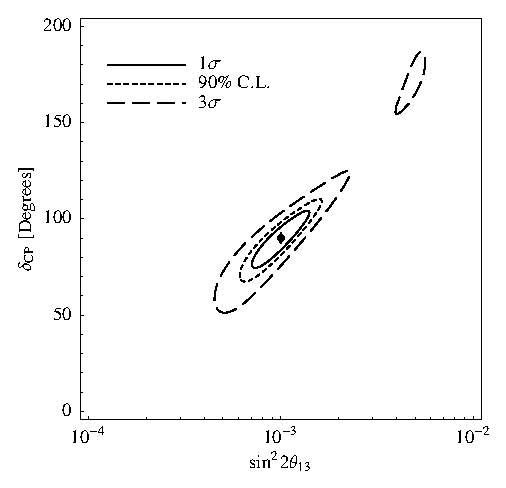
\includegraphics[width=8cm]{correx}}
\end{center}

}

Keeping all oscillation parameters and matter density scaling factors fixed,
 one can use the following functions to obtain the total $\chi^2$ of all 
 specified oscillation channels including systematics:
\begin{function} 
\GLBNS{glbChiSys}
{\tt double glbChiSys(const glb\_params in,int exp, int rule)} returns
the $\chi^2$ for the (fixed) oscillation parameters {\tt in}, the
experiment number {\tt exp}, and the rule number {\tt rule}. For all
experiments or rules, use \GLB{GLB\_ALL} as parameter value.
\end{function}
Note that the result of {\tt glbChiSys} for all experiments or rules
corresponds to the sum of all of the individual {\tt glbChiSys} calls. 
This equality will not hold for the minimizers in the next sections anymore. 
 An example how to use  {\tt glbChiSys} can be found on page~\pageref{ex:corrth13dcp}.  

\index{Systematics} \index{Pull method}
The treatment of systematics in \GLOBES\ is performed by the so-call
{\em pull method} with the help of auxiliary systematics parameters.
They are taken completely uncorrelated among different rules, and treated with simple Gaussian statistics. In general, a rule is a set 
of signal and background event rates coming from different oscillation
channels, where the event rates of all rule contributions are added.
For more details of the rule concept, see \Part~\ref{part:2} of this manual,
and for the treatment of systematics, see \Sec~\ref{sec:rules}.
 
 One example for a systematics parameter the signal normalization error, \ie, an error to the overall normalization of the signal. For illustration, we assume that the signal event rate in the $i$th bin $s_i^0$ of one oscillation channel is altered by the overall normalization auxiliary parameter\index{Auxiliary parameter} of this channel, \ie , 
\be
 s_i = s_i(n_s) = s_i^0 \cdot (1 + n_s),
\ee
where $n_s$ is the signal normalization parameter. The total number of events in the $i$th bin $x_i$ also includes the background event rates $b_i$, \ie, $x_i = s_i + b_i$, which may have their own systematics parameters.
In order to implement an overall signal normalization error $\sigma_{n_s}$,  the $\chi^2$, which includes all event rates $x_i$ of all bins, is minimized over the auxiliary parameter $n_s$:
\be
 \hat{\chi^2} = \underset{n_s}{\mathrm{min}} \left(  \chi^2(n_s, \hdots) + \frac{(n_s)^2}{\sigma_{n_s}^2} \right).
\ee 
This minimization is done independently for all auxiliary parameters of the rule. The total $\chi^2$ for the considered experiment is finally obtained by repeating this procedure for all rules and adding their $\chi^2$-values. In general, the situation is more complicated because of the usage of many systematical errors. More details about systematics parameters and the definition of signal, background, and oscillation channels can be found in \Sec~\ref{sec:rules}, too.

The systematics minimization of an experiment can be easily switched on and off with \GLB{glbSwitchSystematics}, \ie, one can also compute the $\chi^2$ with statistics only. In addition, several options for 
systematics are available, such as only using total event rates without
spectral information. For details, we refer to \Chapt~\ref{chapt:running}.

\chapter[Calculating $\chi^2$-projections: how one can include correlations]{Calculating $\boldsymbol{\chi^2}$-projections: how one can include correlations}
\label{chapt:correlations}
\index{Correlations $\chi^2$}

\index{Multi-parameter correlation}
This chapter deals with the rather complicated issue of $n$-parameter correlations. It is one of the greatest strengths of this software 
to include the full $n$-parameter correlation in the high-dimensional parameter space with reasonable effort. Of course, calculating $\chi^2$-projections is somewhat more complicated than using systematics only. Therefore, we use a simple step by step introduction to the problem. 

\section{Introduction}

\index{Projection of manifold}
In principle, the precision of an individual parameter measurement including correlations in the $\chi^2$-approach can be obtained as the projection of the $n$-dimensional fit manifold onto the respective axis. Similarly, one can project the fit manifold onto a plane, such as the $\stheta$-$\deltacp$-plane, if one wants to explicitely show the allowed
region in this plane with all the other parameter correlations included. 
In practice, this projection is very difficult: a grid-based method would need $(N_{\mathrm{grid}})^n$ function calls of {\tt glbChiSys} to calculate the precision including the full $n$-parameter correlation, where $N_{\mathrm{grid}}$ is the number of points in each direction of the lattice. For example, taking only $N_{\mathrm{grid}}=20$ and $n=7$ (six oscillation parameters and matter density) would mean more than one billion function calls of {\tt glbChiSys}. One can easily image that this is too much for any sophisticated application.

\index{Minimizer}
The solution to this problem is using a local $n$-dimensional (local) minimizer for the projection instead of a grid-based method, where we will
illustrate this minimization process later. It turns out
that such a minimizer can include a full $6$-parameter correlation with of the order of $1\, 000$ function calls of {\tt glbChiSys}. It is a standard method which can be found in every good book for numerical calculation routines. Thus, for each point on the projection axis/plane, one can obtain a result within about $10$ to $30$ seconds on a modern computer, which means that the complete measurement precision for one fixed true parameter set can be obtained in as much as $10$ to $15$ minutes. One can easily imagine that such a minimizer makes more sophisticated applications possible with the help of overnight calculations, such as showing the dependencies on the true parameter values.

This approach also has one major disadvantage: One can not simply program a robust grid-based code and let it run, since using a local minimizer always means that one may end up in an unwanted local minimum and not in the investigated global one. Thus, one has to use some (analytical or numerical) knowledge on the topology of the fit manifold and start the local minimizer close enough to the investigated solution. Fortunately, this can be done quite straightforward in most cases, since the structure of the neutrino oscillation formulas does not cause very complicated topologies of the fit manifolds. Especially the simulation of reactor experiments and conventional beams or superbeams is rather simple with purely numerical
approaches. Neutrino factories have, especially for small values of
$\theta_{13}$, a much more complicated topology. In this case, results
of the many analytical discussions of this issue can be used. This means
 that one can implicitly use the analytical knowledge to obtain better predictions for the measurement performances, since the minimizer has
 to be started only close enough to the exact solution by an ``educated
 guess''. One can easily imagine that the used methods then also depend
 on the region of the parameter space. In this manual, we only use
 examples with a neutrino factory, since some of these complications
 can be illustrated there.

Now, some words of warning with respect to the minimization process: 
Since one can easily find the global fit minimum at the best-fit/simulated values, any additional solution found by the local minimizer makes the measurement performance worse. However, for the real result, the complete
topology has to be taken into account, which means that {\em all} results
fitting the simulated data have to be included, and not only the best-fit
point. Thus, one can only run the danger to obtain a too optimistic solution if one does not find the other local minima appearing below the chosen confidence level. Thus, with this approach and proper usage, it should not possible to produce a too pessimistic solution. 
However, if one is not careful enough to locate
all local minima, one can easily produce too optimistic solutions.
This danger can be summarized as follows:
\begin{equation}
\mathrm{Too \, pessimistic \, result} \, < \, \underbrace{\mathrm{Real \, result}}_{\mathrm{Located \, by \, careful \, usage}} \, \le \, \mathrm{GLoBES \, result} \,  < \,  \mathrm{Too \, optimisitic \, result} \nonumber
\end{equation}

\index{Priors} \index{Input errors} \index{Starting values}
In many cases, the fit manifold is restricted by the knowledge from earlier experiments. For example, the knowledge on the solar parameters will in most cases be supplied by the solar neutrino experiments. If the external precision of a parameter is at the time of the measurement better than the one of the experiment itself, one has to impose some external knowledge on this parameter. This external knowledge may reduce the $n$-dimensional fit manifold in the respective direction. In the most extreme case, keeping all parameters but the measured one fixed in the analysis means that all parameters are determined externally with infinitively high precisions. Thus, using the projection method on the axis/plane of interest is a reasonable approach. The inclusion of external input in \GLOBES\ is done by the use of Gaussian {\em priors}: We assume that an external measurement has determined the measured parameter to be at the central value (which we call {\em starting value}) with a $1 \sigma$ Gaussian error (which we call {\em input error}). The explicit definition of these priors will be shown in the next section. 

\section{The treatment of external input}
\label{sec:externalinput}

\index{External input}
It is one of the strengths of the \GLOBES\ software to use external input in order to reduce the fit manifold with the knowledge from external
(earlier) measurements. The treatment of external input is done by the addition of Gaussian so-called {\em priors} to the systematics-minimized $\chi^2$-function. For example, for the matter density, one obtains as the final projected $\chi^2_F$ after minimization over the matter density
scaling factor \index{Matter density scaling factor} $\hat{\rho}$
\be
 \chi^2_F = \underset{\rho}{\mathrm{min}} \left( \chi^2(\hat{\rho}) + \frac{(\hat{\rho} - \hat{\rho}^0)^2}{\sigma_{\hat{\rho}}^2} \right).
\label{equ:priors}
\ee
This example is a very simple one, since in fact the
minimization is simultaneously performed over all priors and free oscillation parameters. In \equ{priors}, $\hat{\rho}^0$ is the {\em starting value} of the prior, and $\sigma_{\hat{\rho}}$ the $1 \sigma$ absolute (half width) {\em input error}. Thus, it is assumed that an external measurement has determined the matter density with a precision (input error) $\sigma_{\hat{\rho}}$ at the central value $\hat{\rho}^0$. Usually, the starting value is fixed at the best-fit value, and the input error to the $1 \sigma$ half width of the external measurement. For the matter density, $\hat{\rho}^0$  is usually set to $1.0$ corresponding to
the actual matter density profile such as given by the experiment
 definition file, and $\sigma_{\hat{\rho}}$ to the 
relative matter density uncertainty (\eg, $0.05$ for 5\% uncertainty).

In principle, one can set the priors for the matter density and all oscillation parameters. For example, if the disappearance channels of the experiment determine the leading oscillation parameters with unprecedented
precisions, one can omit the respective input errors. In \GLOBES , a
value of $0$ corresponds to neglecting the prior. If, however, earlier external measurements provide better information, one can set their absolute precisions with the input errors. The starting values are usually chosen to be the best-fit values of this external input, such as
for the precisions of the solar experiments. In some cases, it may be
necessary to adjust them, such as for artificial constraints to the
oscillation parameters. In other cases, minor modifications of the starting values can cause a faster convergence of the algorithm.
For example, for the investigation of the
opposite-sign solution, one can use the prior to constrain $\ldm$
in order to force the minimizer not to  fall into the (unwanted) best-fit solution. In this case, the starting value of $\ldm$ would be set to $\rho^0_{\ldm} = - \ldm$, and a $\sigma_{\ldm}$ of the order of $\ldm$ would be imposed. For the algorithm, it would then be rather difficult 
to converge into the unwanted best-fit solution. However, note that one should in this case check that the actually determined value for $\ldm$ after minimization is close enough to the guessed values $-\ldm$ in order to avoid significant artifical contributions of the priors to the 
final $\chi^2$.

\index{Input errors} \index{Starting values}
In order to set the starting values and input errors, two function have to
 be called {\em before the usage of any minimizer}:
\begin{function}
\GLBNS{glbSetStartingValues}
{\tt int glbSetStartingValues(const glb\_params in)} sets the starting values for all of the following minimizer calls to {\tt in}.
\end{function}
\begin{function}
\GLBNS{glbSetInputErrors}
{\tt int glbSetInputErrors(const glb\_params in)}
 sets the input errors for all of the following minimizer calls to {\tt in}.
 An input error of $0$ corresponds to not taking into account the
 respective prior.
\end{function}
Accordingly, there are functions to return the actually set starting values
and input errors:
\begin{function}
\GLBNS{glbGetStartingValues}
{\tt int glbGetStartingValues(glb\_params out)} writes the currently
set starting values to {\tt out}.
\end{function}
\begin{function}
\GLBNS{glbGetInputErrors}
{\tt int glbGetInputErrors(glb\_params out)}
 writes the currently set input errors to {\tt out}.
\end{function}
All functions take or return as many matter density parameters as there are initialized experiments. In addition, they return $-1$ if the operation
was not successful.

\index{External precision}
Eventually, a typical initialization of the external input with
$10\%$ external precisions for the solar parameters\footnote{In fact, accelerator-based long-baseline experiments are primarily sensitive to the product $\sin 2 \theta_{12} \cdot \sdm$, which means that these errors effectively add up to an error of this product of about $15\%$.}, 
and $5\%$ matter density uncertainties for all experiments looks like this:
\begin{quote}
{\tt
 glbDefineParams(input\_errors,theta12*0.1,0,0,0,sdm*0.1,0);\\  
 glbSetDensityParams(input\_errors,0.05,GLB\_ALL);\\
 glbSetStartingValues(true\_values);\\
 glbSetInputErrors(input\_errors);\\
}
\end{quote}
In this example, the starting values are set to the best-fit (simulated) values. Remember that initially the matter density scaling factors are 
all $1.0$, which means that they do not need to be adjusted for the
starting values.

\index{Priors}
\index{Advanced tricks}
Though the priors are an elegant way to treat external input, there are also some complications with priors. The following hints are for the
more advanced \GLOBES\ user:
\begin{enumerate}
\item
 The priors are only added once to the final $\chi^2$, no matter how
 many experiments there are simulated. This is already one reason
 (besides the minimization) why the sum of all projected $\chi^2$'s of 
 the individual experiments 
 cannot correspond to the $\chi^2$ of the combination of all experiments.
\item
 Priors are not used for parameters which are not minimized over, \ie, 
 kept fixed. This will be important together with arbitrary projections
 using \GLB{glbChiNP}. A more subtile consequence is the comparison
 of fit manifold sections and projections for the solutions where
 the absolute minimum $\chi^2$ is larger than zero, \ie, degeneracies
 other than the best-fit solution. In this case, the sections and
 projections are not  comparable if not corrected by the prior contributions, where the
 correction can be obtained as the $\chi^2$-difference at the minimum.
 For example, projecting the $\mathrm{sgn}(\ldm)$-degeneracy onto
 the $\theta_{13}$-$\deltacp$-plane and comparing it with the section
 (all other parameters fixed), the section region would in many cases be 
 larger than the projection region if the priors are not added to the
 section. At the best-fit solution, this problem usually does not occur
 because the prior contributions are close to zero.    
\item
Currently, \GLOBES\ only supports Gaussian priors for the individual
oscillation parameters. Especially for the solar parameters, this is only
 an approximation, since they are imposed on $\theta_{12}$ and not
 on $\sin 2 \theta_{12}$, $\sin 2 \theta_{12} \cdot \sdm$, or $\sin  
 \theta_{12}$. Later versions of  \GLOBES\ may include more alternatives.
 \end{enumerate}
 
 
\example{Projection of two- and $n$-dimensional manifold onto $\stheta$-axis}{
\label{ex:corrproj}
\index{Projection of manifold}
\index{Two-parameter correlation}
\index{Multi-parameter correlation}

This example demonstrates how to project the fit manifold onto the $\stheta$-axis, \ie, how one can include correlations. We compute two sets of data: one for keeping all parameters but $\deltacp$ fixed (two-parameter correlation), and one for keeping all parameters free (multi-parameter correlation). However, we impose external precisions for the solar parameters and the matter density. The following code excerpt is from 
{\tt example2.c}:

\begin{quote}
{\tt {\scriptsize
  /* Set starting values and input errors for all projections */  \\
  glbDefineParams(input\_errors,theta12*0.1,0,0,0,sdm*0.1,0);\\  
  glbSetDensityParams(input\_errors,0.05,GLB\_ALL);\\
  glbSetStartingValues(true\_values);\\
  glbSetInputErrors(input\_errors);\\
\\
  /* Define two-parameter projection: Only deltacp is free! */ \\
  glbDefineProjection(th13\_projection,GLB\_FIXED,GLB\_FIXED,GLB\_FIXED,GLB\_FREE,GLB\_FIXED,GLB\_FIXED); \\
  glbSetProjection(th13\_projection); \\ 
\\
  /* Iteration over all values to be computed */ \\
  double x,res1,res2;     \\
  for(x=-4;x<-2.0+0.001;x=x+2.0/50) \\
  \{ \\
\hspace*{0.5cm}  /* Set fit value of stheta */ \\
\hspace*{0.5cm} glbSetOscParams(test\_values,asin(sqrt(pow(10,x)))/2,1); \\
    \\
\hspace*{0.5cm} /* Guess fit value for deltacp in order to safely find minimum */ \\
\hspace*{0.5cm} glbSetOscParams(test\_values,200.0/2*(x+4)*M\_PI/180,3); \\
 \\
\hspace*{0.5cm} /* Compute Chi2 for user-defined two-parameter correlation */ \\
\hspace*{0.5cm} res1=glbChiNP(test\_values,NULL,GLB\_ALL); \\
      \\
\hspace*{0.5cm} /* Compute Chi2 for full correlation: minimize over all but theta13 */ \\
\hspace*{0.5cm} res2=glbChiTheta(test\_values,NULL,GLB\_ALL); \\
  \\
\hspace*{0.5cm} AddToOutput(x,res1,res2);\\
  \} \\
  
}}
\end{quote}
The two lists of data then represent the $\stheta$ precisions with two-parameter correlations (gray-shaded) and multi-parameter correlations (arrows):
\begin{center}
\colorbox{white}{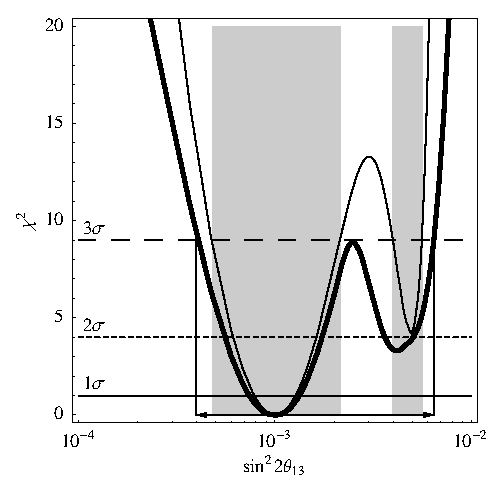
\includegraphics[width=6cm]{projallex}}

\vspace*{0.1cm}

\footnotesize{(Same parameters as on page~\pageref{ex:corrth13dcp} and in \figu{projex}, but 1 d.o.f.)}
\end{center}
}

\section[Projection onto the $\stheta$-axis or $\deltacp$-axis]{Projection onto the $\boldsymbol{\stheta}$- or $\boldsymbol{\deltacp}$-axis}
\index{Projection onto axis}

\begin{figure}[t]
\begin{center}
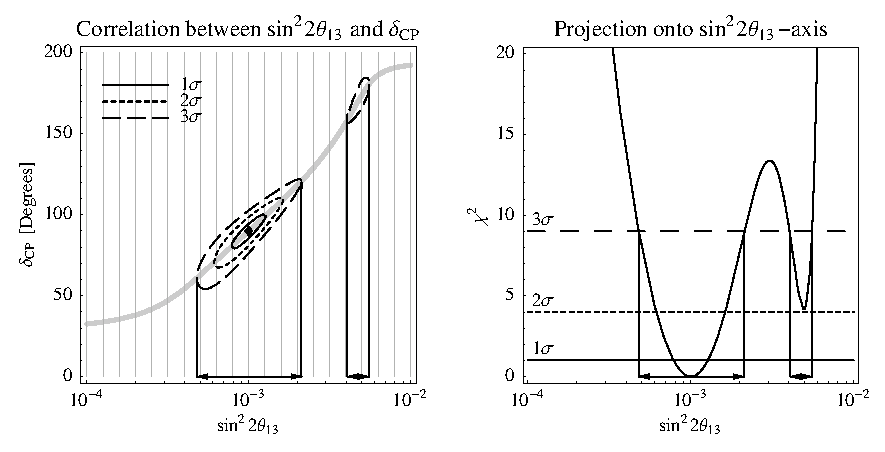
\includegraphics[width=16cm]{projex}
\end{center}
\mycaption{\label{fig:projex} Left plot: The correlation between $\stheta$ and $\deltacp$ as calculated in the example on page~\pageref{ex:corrth13dcp}, but for 1 d.o.f. only. Right plot: The $\chi^2$-value of the projection onto the $\stheta$-axis as function of $\stheta$. The projection onto the  $\stheta$-axis is obtained by finding the minimum $\chi^2$-value for each fixed value of $\stheta$ in the left-hand plot, \ie, along the gray vertical lines. The thick gray curve marks the position of these minima in the left-hand plot. The arrows mark the obtained fit ranges for $\stheta$ at the $3 \sigma$ confidence level (1 d.o.f.), \ie , the precision of $\stheta$.}
\end{figure}

The projection onto the $\stheta$- (or $\deltacp$-) axis is performed by fixing $\stheta$ (or $\deltacp$) and minimizing the $\chi^2$-function over all free fit parameters and the matter densities. We illustrate this method at the example of the projection of the two-dimensional manifold in the $\stheta$-$\deltacp$-plane onto the $\stheta$-axis in \figu{projex}. In this figure, the left-hand plot shows the correlation in the $\stheta$-$\deltacp$-plane computed with {\tt glbChiSys}. The right-hand plot illustrates the projection of this two-dimensional manifold onto the $\stheta$ axis by minimizing $\chi^2$ over $\deltacp$. In this simple example, the minimization is done along the vertical gray lines in the left hand plot. The obtained minima are located on the thick gray curve, which means the the right-hand plot represents the $\chi^2$-value along this curve. In fact, one can easily see that one obtains the correct projected $3 \sigma$ errors in this example (\cf, arrows). This figure illustrates the projection of a two-parameter correlation. In general, the full $n$-parameter correlation is treated similarly by the simultaneous (local) minimization over all free fit parameters. 

\index{Minimizer}
The following functions are some of the simplest minimizers 
provided by \GLOBES :
\begin{function}
\GLBNS{glbChiTheta}
{\tt double glbChiTheta(const glb\_params in, glb\_params out, int exp)}
returns the projected $\chi^2$ onto the $\theta_{13}$-axis for the  experiment {\tt exp}. For the simulation of all initialized experiments,
use {\tt GLB\_ALL} for {\tt exp}. The values in {\tt in} are the guessed fit values for the minimizer (all parameters other than $\theta_{13}$) and the fixed fit value of $\theta_{13}$. The actually determined parameters at the minimum are returned in {\tt out}, where $\theta_{13}$ is still at
its fixed value. If {\tt out} is set to {\tt NULL}, this information will not be returned.
\end{function}
\begin{function}
\GLBNS{glbChiDelta}
{\tt double glbChiDelta(const glb\_params in, glb\_params out, int exp)}
returns the projected $\chi^2$ onto the $\deltacp$-axis for the  experiment {\tt exp}. For the simulation of all initialized experiments,
use {\tt GLB\_ALL} for {\tt exp}. The values in {\tt in} are the guessed fit values for the minimizer (all parameters other than $\deltacp$) and the fixed fit value of $\deltacp$. The actually determined parameters at the minimum are returned in {\tt out}, where $\deltacp$ is still at its fixed value. If {\tt out} is set to {\tt NULL}, this information will not be returned.
\end{function}

All of the minimization functions have a similar parameter structure: The fixed fit parameter value and the guessed starting point of the minimizer, \ie, the guessed position of the minimum, are transferred in the list {\tt in}. Part of this list are the matter density
scaling factors of all experiments, which are also minimized over. 
The minimizer is then started at the guessed point and runs into
the local minimum, where the fit parameter of the projection
axis is fixed. For the best-fit solution, it is usually sufficient to start the minimizer at the best-fit point. However, the convergence speed might
be better by starting it slightly off this point. In addition, there
are problems in many cases with more complicated topologies, which means
that better guesses for the position of the minimum are needed.
The position of the minimum is then returned in {\tt out}
together with the number of iterations used for the minimization.
It is very often useful to print the output of the minimization with
\GLB{glbPrintParams} in order to check that the minimum is the
appropriate one. For example, if the minimizer ends up in the wrong-sign
solution in $\ldm$, priors can be used to force it into the tested
minimum. In addition, the number of iterations used allows an optimization
of the convergence speed. 
% 
Note that before any minimization, \GLB{glbSetStartingValues} 
and \GLB{glbSetInputErrors} have to be used at least once. In addition, note that the resulting $\chi^2$ of {\tt glbChiTheta} (or {\tt glbChiDelta}) for the combination of more than one experiment is not 
equal to the sum of the individual $\chi^2$-values anymore. This has two reasons: First, the topology of the fit manifold is altered by the addition of $\chi^2$-values of different experiments. Thus, after the minimization, the position of the minimum can be different to the ones of the individual experiments. Second, the priors for the external knowledge on the parameters are only added once -- independent of the number of experiments.

\index{Matter density scaling factor}
The the output of the minimizer in {\tt out} carries as many matter density scaling factors as there are experiments. Either
one (for the simulation of one experiment) or all (for the simulation of
all experiments) are different from $1.0$ if matter density uncertainties
are present, since each experiment may face other matter density conditions. The minimizer for individual experiments ``know'' which
experiment they are currently treating, which means that only the returned
matter density scaling factor of the appropriate experiment is modified.
For example, calculating {\tt glbChiTheta} for the last experiment
number, the last density values will be modified.
This approach turns out to be extremely useful together with the
simulation of more than one experiment. One can, for instance, locate the
degeneracies of all individual experiments. In order to test if
these degeneracies are still present in the combination of all experiments (which has a very different topology), one can test the combination of experiments with the output {\tt out} from the individual experiments. In this case, even the correct matter density scaling factor
output is used. 

The example on page~\pageref{ex:corrproj} demonstrates how one can obtain \figu{projex} (right) with keeping all parameters but $\deltacp$ fixed, as well as how one can include the full $n$-parameter correlation with external input. It also demonstrates how these two compare to each other. One can easily read off this example that 
there is a substantial impact of the
correlation with oscillation parameters other than $\deltacp$. 
Note that it uses the function
\GLB{glbChiNP} for arbitrary projections from the next section for the minimization over $\deltacp$.
In addition, there is one interesting feature in guessing the
oscillation parameters in this example: In order to avoid falling
into the wrong minimum, the fit value of $\deltacp$ is guessed from \figu{projex} (left). This quite sophisticated ``guessing'' is typical
for neutrino factories because of the $(\deltacp, \theta_{13})$-degeneracy, whereas it is for superbeams often sufficient
to use the best-fit values. A strong indication for a wrong guessing 
are discontinuous jumps in the projected $\chi^2$-function, where the minimizer jumps from one minimum to another. In such cases, the starting point of the minimizer has to be adjusted to help it find the true minimum.

Other examples for projections onto a parameter axis while keeping exactly one parameter fixed are \GLB{glbChiTheta23}, \GLB{glbChiDm}, and \GLB{glbChiDms}, which
can be found in \Tab~\ref{tab:stdfunctions} on page~\pageref{tab:stdfunctions}.

\section[Projection onto any hyperplane]{Projection onto any hyperplane}
\index{Projection onto hyperplane}

In general, one can show the measurement result in any $k$-dimensional hyperplane, where $k$ is smaller than the dimension of the parameter space $n$, and thus the dimension of the fit manifold. In this case, $k$ parameters are fixed and $n-k$ parameters are minimized over. One such example is the projection of the fit manifold onto the $\stheta$-$\deltacp$-plane, \ie, $k=2$ here. In this case, the two
parameters $\stheta$ and $\deltacp$ are kept fixed, and the others are
minimized over. 
The corresponding function is \index{Projection onto $\theta_{13}$-$\deltacp$-plane}
\begin{function}
\GLBNS{glbChiThetaDelta}
{\tt double glbChiThetaDelta(const glb\_params in, glb\_params out, int exp)} returns the projected $\chi^2$ onto the $\theta_{13}$-$\deltacp$-plane for the  experiment {\tt exp}. For the simulation of all initialized experiments,
use {\tt GLB\_ALL} for {\tt exp}. The values in {\tt in} are the guessed fit values for the minimizer (all parameters other than $\theta_{13}$ and $\deltacp$) and the fixed fit values of $\theta_{13}$ and $\deltacp$. The actually determined parameters at the minimum are returned in {\tt out}, where $\theta_{13}$ and $\deltacp$ are still at their fixed values. If {\tt out} is set to {\tt NULL}, this information will not be returned.
\end{function}
This function works analogously to the ones in the last section. They can, for example, be used to obtain a figure similar to \figu{projex}, left.
The example on page~\pageref{ex:corrproj} illustrates then the difference
between the projections of the ``eggs'' within the 
$\stheta$-$\deltacp$-plane onto the $\theta_{13}$-axis. 
Though the running time for one call of these functions is somewhat 
shorter than the one for the $\stheta$- or $\deltacp$-projections, one 
has to compute a two-dimensional array for such a figure (instead of a 
one-dimensional list). Therefore, the overall computational effort is 
much higher, \ie, in the order of hours. In many cases, it is therefore
convenient to run {\tt glbChiSys} first to obtain a picture of
the manifold and to adjust the parameter ranges. Then, one can run
{\tt glbChiThetaDelta} for a complete evaluation of the problem
including correlations.

\begin{table}[t!]
\begin{tabular}{p{4.2cm}p{5.5cm}p{5.1cm}}
\hline
Function & Purpose & Parameters $\rightarrow$ Result\\
\hline
\GLB{glbAllocProjection} & Create projection vector & {\tt ()} \\
\GLB{glbFreeProjection} & Destroy projection vector {\tt stale} & {\tt (glb\_projection stale)} \\
\GLB{glbDefineProjection} & Assign projection vector {\tt in} & {\tt (glb\_projection in, int theta12, int theta13, int theta23, int delta, int dms, int dma)} \\ 
\GLB{glbCopyProjection} & Copy vector {\tt source} to {\tt dest} & {\tt (const glb\_projection source, glb\_projection dest)} \\
\GLB{glbPrintProjection} & Print vector {\tt in} to file {\tt stream} & {\tt (FILE* stream, const glb\_projection in)} \\
\GLB{glbSetProjectionFlag} & Set flag for oscillation parameter {\tt which} in vector {\tt in} to value {\tt flag}. & {\tt (glb\_projection in, int flag, int which)} \\
\GLB{glbGetProjectionFlag} & Return flag for oscillation parameter {\tt which} in vector {\tt in}. & {\tt (const glb\_projection in, int which)} $\rightarrow$ {\tt int} flag \\
 {\tt glbSetDensity\-ProjectionFlag} \GLBNS{glbSetDensityProjectionFlag} & Set flag for density parameter {\tt which} in vector {\tt in} to value {\tt flag}. & {\tt (glb\_projection in, int flag, int which)} \\
{\tt glbGetDensity\-ProjectionFlag} \GLBNS{glbGetDensityProjectionFlag} & Return flag for density parameter {\tt which} in vector {\tt in}.  & {\tt (const glb\_projection in, int which)} $\rightarrow$ {\tt int} flag \\
\hline
\end{tabular}
\caption{\label{tab:defprojection}\index{Projection type}
Different functions handling the
\GLB{glb\_projection} type. Flags are either \GLB{GLB\_FIXED} or \GLB{GLB\_FREE}. The (un-shown) return values of the {\tt Set-} and {\tt Define-} functions point either to the assigned vector if successful, or they are {\tt NULL} if unsuccessful.}
\end{table}

In principle, one can also use three- or more-dimensional projections. In addition, one may want to use a different set of parameters for single- or two-parameter projections. The very flexible function \GLB{glbChiNP} is
designed for this purpose. However, because of its flexibility, it 
involves more sophistication.

In order to define arbitrary projections, we introduce the vector
\GLB{glb\_projection}, which is very similar to the
oscillation parameter vector {\tt glb\_params}.
Normally, the user does not need to access this type directly:
A set of function similar to the ones for {\tt glb\_params} is
provided. The purpose of {\tt glb\_projection} is to tell \GLOBES\ 
what parameters are fixed, and what are minimized over. Thus, in
comparison to {\tt glb\_params}, it does not take values for the
parameters, but flags \GLB{GLB\_FIXED} or \GLB{GLB\_FREE}.
For example, the projection onto the $\theta_{13}$-axis {\tt glbChiTheta}
is nothing else than a special case of {\tt glbChiNP} with $\theta_{13}$
fixed and all the other parameters free. Similar to {\tt glb\_params},
the type {\tt glb\_projection} has to be created first, and destroyed
later. The access functions for {\tt glb\_projection} are summarized in \Tab~\ref{tab:defprojection}. Since the complete set is very similar to
the one for {\tt glb\_params}, we do not go into greater details here.

\index{Projection: Define}
As soon as we have defined a projection, we can assign it:
\begin{function}
\GLBNS{glbSetProjection}
{\tt int glbSetProjection(const glb\_projection in)} sets the projection
to {\tt in}. The return value is $0$ if successful, and $-1$ if
unsuccessful.
\end{function}
Similarly, the currently assigned projection can be returned with:
\begin{function}
\GLBNS{glbGetProjection}
{\tt int glbGetProjection(glb\_projection out)} writes the currently
set projection to {\tt out}. The return value is $0$ if successful, and $-1$ if unsuccessful.
\end{function}
After setting the starting values, input errors, and the projection, 
we can run the minimizer:
\begin{function}
\GLBNS{glbChiNP}
{\tt double glbChiNP(const glb\_params in, glb\_params out, int exp)} 
returns the projected $\chi^2$ onto the hyperplane specified by 
{\tt glbSetProjection} for the  experiment {\tt exp}. 
For the simulation of all initialized experiments,
use {\tt GLB\_ALL} for {\tt exp}. The values in {\tt in} are the guessed fit values for the minimizer (all free parameters) and the fit values
on the hyperplane (all fixed parameters). The actually determined parameters at the minimum are returned in {\tt out}, where the fixed parameters are still at their input values. If {\tt out} is set to {\tt NULL}, this information will not be returned.
\end{function}
As an example, the projection sequence for a minimization over
$\deltacp$ only looks like this:
\begin{quote}
{\tt
  glb\_projection th13\_projection = glbAllocProjection(); \\
  glbDefineProjection(th13\_projection,GLB\_FIXED,GLB\_FIXED,GLB\_FIXED,\\
  \hspace*{2cm} GLB\_FREE,GLB\_FIXED,GLB\_FIXED); \\
  glbSetProjection(th13\_projection); \\ 
  res1=glbChiNP(test\_values,NULL,GLB\_ALL); \\
  glbFreeProjection(th13\_projection);
}
\end{quote}
In this case, only the correlation with $\deltacp$ is taken into account.
Note that in the  example on page~\pageref{ex:corrproj} this projection
is compared with the result including the full multi-parameter correlation.

\chapter{Locating degenerate solutions}
\index{Degenerate solutions}
\index{Degeneracies $\chi^2$}

In the last chapter, we introduced the projection of any set of $k$ parameter onto any $n-k$ dimensional hyperplane, which was done by the minimization over the $k$ free fit parameters. Similarly, one can minimize over {\em all} $n$ parameters to find the local minimum close to any starting point. This approach is very useful for the exact numerical location of a degeneracy if its approximate position is known. For the determination of the approximate position, one can use analytical approaches or an educated guess. 
Though the usage of the all-parameter minimizers is quite simple, one should keep in mind that they are local minimizers. Therefore, one may need a very sophisticated application software to find all degenerate solutions.

\example{Finding the $\mathrm{sgn}(\ldm)$-degeneracy}{
\label{ex:sgndeg}
\index{Degeneracies: sgn($\ldm$)-degeneracy}

In many cases, one can find the exact position of the $\mathrm{sgn}(\ldm)$-degeneracy with \GLB{glbChiAll}, where one starts 
the local minimizer at the suspected position 
and let it converge into the minimum.  The following code excerpt  corresponds to finding the degenerate solution for the example on
  page~\pageref{ex:corrth13dcp}, and it is from {\tt example3.c}: 
\begin{quote}
{\tt
{\footnotesize
  /* Set starting vales to suspected position at opposite sign of ldm */ \\
  \mbox{glbDefineParams(starting\_values,theta12,theta13,theta23,deltacp,sdm,-ldm);} \\
  \\
  /* Set input errors for external input, where some information on ldm \\
   \hspace*{0.5cm} is imposed in order to avoid falling into the right-sign solution */ \\
  glbDefineParams(input\_errors,theta12*0.1,0,0,0,sdm*0.1,ldm/3); \\ 
  glbSetDensityParams(input\_errors,0.05,GLB\_ALL); \\
  \\
  glbSetStartingValues(starting\_values); \\
  glbSetInputErrors(input\_errors); \\
  \\
  /* Localize degenerate solution by minimization over all parameters */ \\
  double CL=glbChiAll(starting\_values,deg\_pos,GLB\_ALL); \\
   \\
  \mbox{/* Now: CL is the chi2 of the deg.~solution and deg\_pos the position */} 
}}
\end{quote}

Using {\tt ent\_pos} to obtain a section of the degeneracy in the
$\stheta$-$\deltacp$-plane (\cf, {\tt example3.c}), one can plot it as a contour plot in addition to the original solution (2 d.o.f., gray curves):
\begin{center}
\colorbox{white}{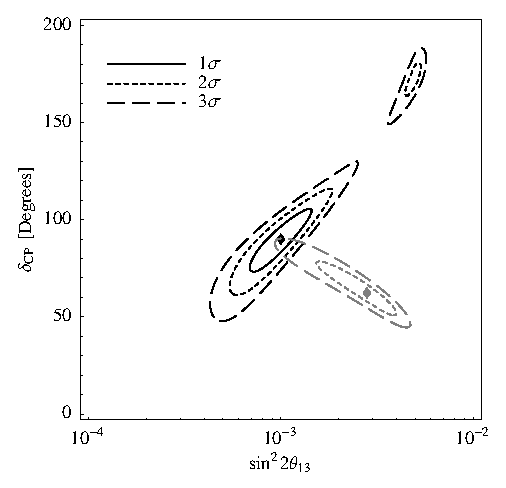
\includegraphics[width=7.5cm]{correntex}}
\end{center}

}

\index{All-parameter minimization}
The function to perform the all-parameter minimization is {\tt glbChiAll}:
\begin{function}
\GLBNS{glbChiAll} 
{\tt double glbChiAll(const glb\_params in, glb\_params out, int exp)}
  returns the minimized $\chi^2$ over all parameters for the  experiment {\tt exp}. For the simulation of all initialized experiments,
use {\tt GLB\_ALL} for {\tt exp}. The values in {\tt in} are the guessed fit values for the minimizer. The actually determined parameters at the minimum are returned in {\tt out}. If {\tt out} is set to {\tt NULL}, this information will not be returned.
\end{function}
%
This function takes the suspected position of the local minimum and returns its actual position in {\tt out}, as well as the $\chi^2$-value 
at the minimum as return value. Thus, the return value can be immediately
used to judge whether the located degeneracy appears at the chosen
confidence level.

The example on page~\pageref{ex:sgndeg} illustrates how to locate the $\mathrm{sgn}(\ldm)$-degeneracy and show the corresponding degenerate solution in the $\stheta$-$\deltacp$-plane together with the original solution.
In this case, the position of the degeneracy can be easily guessed to be at the best-fit parameter values but the $\ldm$ inverted. The minimizer then runs off the plane of the best-fit parameters into the local minimum. It is very important to take into account the position of the degeneracy off this plane, since the actual $\chi^2$ in the minimum is certainly lower than on the plane of the best-fit parameter values. Thus, the degeneracy may not even appear at the chosen confidence level on the plane, but it does appear at the true minimum. The two sections\footnote{The discussed figure on page~\pageref{ex:sgndeg} is produced by  {\tt glbChiSys} and thus only represents a section through the fit manifold. For the projection including correlations, one may rather want to use {\tt glbChiThetaDelta}.} through the fit manifold shown in the figure on page~\pageref{ex:sgndeg} therefore do not appear at the same oscillation parameter values (except from the ones shown in the figure). 

\index{Advanced tricks}
For the more advanced reader, a number of tricks can be useful for the numerical localization of degenerate solutions:
\begin{description}
\item[Minimum $\boldsymbol{\chi^2}$ larger than threshold.] If a located degeneracy has a minimum $\chi^2$ larger than the corresponding confidence level threshold for the discussed quantity of interest, the degeneracy can be immediately ignored. This saves a lot of computation time.
\item[Locating degeneracies in more complicated topologies.] For more complicated topologies, such as for neutrino factories, it is often useful to use multi-step location procedures or analytical knowledge. For example, for a numerical procedure, one may first of all switch off the systematics and keep $\stheta$ or $\deltacp$ fixed, \ie, use {\tt glbChiTheta}, where $\stheta$ or $\deltacp$ is fixed at the best-fit value. The result can then be used as a starting point for {\tt glbChiAll} for the individual experiments with the systematics switched on again. 
\item[Forcing the minimizer into the targeted solution.]
In addition to switching off the systematics, it can be useful to reduce the input errors during some steps of the localization process in order to make the minimizer not to run away too much from the targeted solution.
The example on page~\pageref{ex:sgndeg} illustrates this with the
input error for $\ldm$: Since the guessed starting point might be
quite far away from the real degeneracy, the algorithm may in some cases
find the original solution instead of the degeneracy (which can
be immediately seen from the output vector). The input error
for $\ldm$ gives the algorithm a ``bias'' against the original solution.
However, note that the input error must not be too small in order
to avoid a significant contribution of the prior to the final $\chi^2$.
Alternatively, one could run {\tt glbChiAll} again with the located minimum
as {\tt in} vector and $\ldm$ kept free.
\item[Finding degeneracies with multiple experiments.] For multiple experiments, it turns out to be useful to locate the degeneracies for individual experiments first. Then, all of the found degeneracies below the threshold can be tested for the combination of all experiments.
\end{description}
Finally, note that any degenerate solution below the confidence level threshold which can not be located makes the result appear better than it actually is. Thus, one should be careful with the determination of the degenerate solutions in order to find all of them.

\chapter{Obtaining low-level information}
\index{Low-level information}

In this chapter, we discuss possibilities to obtain low-level information
in \GLOBES , \ie, about oscillation probabilities, rates, and other
information lower than on the $\chi^2$-level.

\section{Oscillation probabilities}
\index{Oscillation probabilities}

\GLOBES\ can compute the probabilities in vacuum
with the following function:
\begin{function}
\GLBNS{glbVacuumProbability}
{\tt double glbVacuumProbability(int l, int m, int panti,double E, double L)} returns the neutrino oscillation probability $\nu_l \rightarrow \nu_m$ for the energy {\tt E} and the baseline {\tt L} in vacuum. The parameter
{\tt panti} is $+1$ for neutrinos and $-1$ for antineutrinos. 
\end{function}
In addition, the oscillation probabilities in matter can be obtained
with:
\begin{function}
\GLBNS{glbProfileProbability}
{\tt double glbProfileProbability(int l, int m, int panti,double E)}
 returns the neutrino oscillation probability $\nu_l \rightarrow \nu_m$ for the energy {\tt E} in matter. The parameter
{\tt panti} is $+1$ for neutrinos and $-1$ for antineutrinos.
The matter density profile including baseline is the one from the last
evaluated experiment. 
\end{function}
THIS FUNCTION MAY OBTAIN AN EXPERIMENT INDEX (WW).
\section{Event rates}
\index{Event rates}
One can also return event rates in \GLOBES , but this feature
requires some knowledge about the experiment definition. 
In fact, many of these functions are very advanced, which means
that the reader who wants to use them should be familiar with
\Secs~\ref{sec:channel} and~\Sec~\ref{sec:rules} of the \AEDL\ manual.

\index{Event rates}
\GLOBES\ currently supports rule-based and channel-based event rate functions, where the information is in written into a file
or returned in a list. The rule-based functions are:
\begin{function}
\GLBNS{glbShowRuleRates}
{\tt int glbShowRuleRates(FILE* stream, int exp, int rule, int pos,
int effi, int bgi, int coeffi, int signal)} prints the binned rule rates as
list with energy and event rate to the file {\tt stream} (either an
open file, or {\tt stdout}). A specific experiment {\tt exp} and a 
specific rule {\tt rule} have to be chosen, as well as the signal
or background rate {\tt signal} (either \GLB{GLB\_SIG} or \GLB{GLB\_BG}).
The position {\tt pos} refers to the component within the signal or 
background, and can also be {\tt GLB\_ALL}. The function may return
the rates with (\GLB{GLB\_W\_COEFF}) or without (\GLB{GLB\_WO\_COEFF})
overall efficiency coefficient, as it is specified by {\tt coeffi}. 
In addition, it may contain the post-smearing efficiencies (set
{\tt effi} to \GLB{GLB\_W\_EFF} or \GLB{GLB\_WO\_EFF}), and the
post-smearing backgrounds (set
{\tt bgi} to \GLB{GLB\_W\_BG} or \GLB{GLB\_WO\_BG}). The pre-smearing
efficiencies and backgrounds cannot be accessed at the rule level.
The return value
is $0$ if successful, and $-1$ if unsuccessful.
\end{function}
\begin{function}
\GLBNS{glbTotalRuleRate}
{\tt double glbTotalRuleRate(int exp, int rule, int pos,
int effi, int bgi, int coeffi, int signal)} returns the total rates with
the same parameters as {\tt glbShowRuleRates}.
\end{function}
The function {\tt glbTotalRuleRate} is especially useful if
one wants to draw bi-rate graphs with total event rates, or look
for the $(\deltacp,\theta_{13})$-degeneracy by the intersection of 
neutrino and antineutrino constant event rate curves.
%
In order to obtain information on the structure of the rules, 
a number of additional functions are provided:
\begin{function}
\GLBNS{glbGetNumberOfRules}
{\tt int glbGetNumberOfRules(int exp)} returns the number of
rules in experiment {\tt exp}.
\end{function}
\begin{function}
\GLBNS{glbGetLengthOfRule}
{\tt int glbGetLengthOfRule(int exp, int rule, int signal)} returns
the length of rule {\tt rule} in experiment {\tt exp}. The parameter
{\tt signal} can be either \GLB{GLB\_SIG} for the number of signal
components or \GLB{GLB\_BG} for the number of background components.
\end{function}
\begin{function}
\GLBNS{glbGetNormalizationInRule}
{\tt double glbGetNormalizationInRule(int exp, int rule, int signal)}
returns the normalization (normalization or background center)
in rule {\tt rule} of the experiment {\tt exp}.
The parameter {\tt signal} refers to signal (\GLB{GLB\_SIG}) or background
(\GLB{GLB\_BG}).
\end{function}
\begin{function}
\GLBNS{glbGetChannelInRule}
{\tt int glbGetChannelInRule(int exp, int rule, int pos, int signal)}
returns the channel number in rule {\tt rule} at the position {\tt pos}
of the experiment {\tt exp}.
The parameter {\tt signal} refers to signal (\GLB{GLB\_SIG}) or background
(\GLB{GLB\_BG}).
\end{function}
\begin{function}
\GLBNS{glbGetCoefficientInRule}
{\tt double glbGetCoefficientInRule(int exp, int rule, int pos, int signal)}
returns the coefficient of the component {\tt pos} in rule {\tt rule} 
of the experiment {\tt exp}.
The parameter {\tt signal} refers to signal (\GLB{GLB\_SIG}) or background
(\GLB{GLB\_BG}).
\end{function}


In addition, \GLOBES\ has channel-based rate functions:
\begin{function}
\GLBNS{glbShowChannelRates}
{\tt int glbShowChannelRates(FILE *stream,
int exp, int channel, int smearing, int effi, int bgi)}
prints the binned channel rates as
list with energy and event rate to the file {\tt stream} (either an
open file, or {\tt stdout}). A specific experiment {\tt exp} and a 
specific channel {\tt channel} have to be chosen.
The function may return
the rates before (\GLB{GLB\_PRE}) or after (\GLB{GLB\_POST})
the energy smearing, as it is specified by {\tt smearing}.
In addition, it may contain the pre- and post-smearing efficiencies (set
{\tt effi} to \GLB{GLB\_W\_EFF} or \GLB{GLB\_WO\_EFF}), and the
pre- and post-smearing backgrounds (set
{\tt bgi} to \GLB{GLB\_W\_BG} or \GLB{GLB\_WO\_BG}). Note that
the post-smearing efficiencies and backgrounds cannot be taken into
account if the rates are returned before the energy smearing.
The return value
is $0$ if successful, and $-1$ if unsuccessful.
\end{function}
\begin{function}
\GLBNS{glbGetChannelRates}
{\tt int glbGetChannelRates(double** data,
size\_t* length, int exp, int channel, int smearing)}
writes the binned raw channel rates to the list {\tt data}
and the length of this list to {\tt length}. 
A specific experiment {\tt exp} and a 
specific channel {\tt channel} have to be chosen.
The function may return
the rates before ({\tt smearing} is \GLB{GLB\_PRE}) or after ({\tt smearing} is \GLB{GLB\_POST})
the energy smearing, where no user-defined data
(pre-/post-smearing efficiencies or backgrounds) are taken into account.
The return value is $-1$ if unsuccessful.
\end{function}
\begin{function}
\GLBNS{glbGetUserData}
{\tt int glbGetUserData(double** data,
size\_t* length, int exp, int channel, int smearing, int bgeff)}
writes the binned user-defined backgrounds or efficiencies 
to the list {\tt data} and the length of this list to {\tt length}. 
A specific experiment {\tt exp} and a 
specific channel {\tt channel} have to be chosen.
The function may return
the pre- ({\tt smearing} is \GLB{GLB\_PRE}) or post- ({\tt smearing} is \GLB{GLB\_POST}) smearing backgrounds ({\tt bgeff} is \GLB{GLB\_BG}) 
or efficiencies ({\tt bgeff} is \GLB{GLB\_EFF}). 
The return value is $-1$ if unsuccessful.
\end{function}
Since \GLOBES\ reserved the memory for the lists returned in these
functions, which it allocates on an internal stack, one has to reset
the stack at the end of the rates access with
\begin{function}
\GLBNS{glbResetRateStack}
{\tt void glbResetRateStack()} resets the rate stack used for the
lists returned from {\tt glbGetChannelRates} or {\tt glbGetUserData}.
\end{function}
A code excerpt to show the channel rates may look like this:
\begin{quote}
{\tt
 double* rates; \\
  size\_t length; \\
  glbGetChannelRates(\&rates,\&length,0,0,GLB\_PRE); \\
  int i; \\
  for(i=0;i<length;i++) printf("\%g $\backslash$n",rates[i]); \\
  glbResetRateStack(); \\
}
\end{quote}
Finally, one can find the number of channels of an experiment:
\begin{function}
\GLBNS{glbGetNumberOfChannels}
{\tt int glbGetNumberOfChannels(int exp)} returns the number of 
channels of experiment {\tt exp}.
\end{function}

\section{Fluxes and cross sections}
\index{Flux} \index{Cross section}

Another piece of low-level information, which can be returned by \GLOBES ,
are the numbers from the loaded fluxes and cross sections.
The following functions interpolate on the loaded fluxes and cross 
sections, \ie, any value in the allowed energy range can be given as input:
\begin{function}
\GLBNS{glbFlux}
{\tt double glbFlux(int exp, int ident, 
double E, double distance, int l, int anti)} returns
the flux of flux number {\tt ident} of the experiment {\tt exp}
for the flavor $\nu_l$ 
and polarity {\tt anti} ($+1$: neutrinos, $-1$: antineutrinos) at the energy {\tt E} and distance {\tt distance}.
\end{function}

\begin{function}
\GLBNS{glbXSection}
{\tt double glbXSection(int exp, 
int ident, double E, int l, int anti)} returns
the cross section of experiment {\tt exp}, 
cross section number {\tt ident} for the flavor $\nu_l$ and polarity {\tt anti} ($+1$: neutrinos, $-1$: antineutinos) at the energy {\tt E}.
\end{function}
Note that all flux or flavor numbers run from $0$ to $N-1$ in these functions.

\chapter{Changing experiment parameters at running time}
\label{chapt:running}
\index{Experiment parameters}

Many of the parameters in experiment definitions can be changed
at running time. For example, we have introduced in 
\Sec~\ref{sec:luminosity} possibilities to change the integrated
luminosity, which consists of source power, running time, and target mass.
In this chapter, we discuss more sophisticated
experiment changes. However, since \GLOBES\ computes a lot of
information only once when an experiment is loaded, many
parameters can not be changed at running time. For example,
the energy resolution function or the number of bins are used
to compute the smearing matrix already at the initialization
of the experiment, which saves a lot of computation
time for most applications. In \Sec~\ref{sec:aedlparams}, we 
introduce a mechanism how one can even change these \AEDL\ parameters
during running time.

\section{Baseline and matter density profile}
\index{Baseline: Change}
\index{Matter density profile: Change}

In order to change the baseline of an experiment, it is important
to keep in mind that each experiment has a profile type defined
in the \AEDL\ file (average density, PREM profile with a given
number of steps, or arbitrary profile). One can check the currently
used profile type with
\begin{function}
\GLBNS{glbGetProfileType}
{\tt int glbGetProfileType(int exp)} returns the matter density profile
type of experiment {\tt exp}.
\end{function}
For each profile type, one can easily change the baseline with {\tt glbSetBaselineInExperiment},
where the average density or the PREM profile are re-computed, or the
steps in the arbitrary profile are re-scaled. Of course, though this
function is sufficient in most cases, it does often not make sense
for arbitrary matter density profiles.
\begin{function}
\GLBNS{glbSetBaselineInExperiment}
{\tt int glbSetBaselineInExperiment(int exp, double baseline)}
sets the baseline length in experiment {\tt exp} to {\tt baseline}.
The function returns $-1$ if it was not successful.
\end{function}
Note that {\tt glbSetBaselineInExperiment} does not change the
profile type in the experiment. The counterpart of this function is:
\begin{function}
\GLBNS{glbGetBaselineInExperiment} 
{\tt double glbGetBaselineInExperiment(int exp)} returns the
baseline length currently used for experiment {\tt exp}.
\end{function}
One can not change the profile type of an experiment manually
during running time. However, one can change the matter density
profile, where the profile type is automatically changed to three
(arbitrary matter density profile). In addition, a number of functions 
are provided to compute possible matter density profiles (average density,
PREM profile). In general, a matter density profile in \GLOBES\ with
$N$ layers is represented by a list of lengths 
\begin{equation}
\mathrm{Lengths} = (x_1,x_2, \hdots, x_N) 
\end{equation}
and a list of densities
\begin{equation}
\mathrm{Densities} = (\rho_1,\rho_2, \hdots, \rho_N), 
\end{equation}
where the baseline is given by
\begin{equation}
L = \sum\limits_{i=1}^N x_i.
\end{equation}
In C, lists are represented as pointers to the first element:
\begin{quote}
{\tt  
  double* lengths; \\
  double* densities;
}
\end{quote}
Many of the \GLOBES\ baseline functions take and return
such lists as parameters, and are therefore more sophisticated
to handle. In general, any function
{\em returning} lists reserves the memory space for them.
It is then up to the user to return the allocated memory!
In addition, they normally return the length of the lists $N$
in form of a pointer, where the corresponding memory space 
has to be provided by the user (normally, it is enough to declare
a variable of the type {\tt size\_t} corresponding to positive
integer numbers).
The following functions return matter density profiles:
\begin{function}
\GLBNS{glbLoadProfileData}
{\tt int glbLoadProfileData(const char* filename, size\_t *layers, double **lengths, double **densities)} loads a density file from the file
{\tt filename}. It returns the number of layers {\tt layers}, the
list of lengths {\tt lengths}, and the list of densities {\tt densities}.
\end{function}
The file should contain in each line a length and density for one layer,
which are separated by an empty space.
\begin{function}
\GLBNS{glbStaceyProfile}
{\tt int glbStaceyProfile(double baseline, size\_t layers, double **lengths, double **densities)} creates a PREM/Stacey matter density profile with a
number of {\tt layers} steps for the baseline {\tt baseline}. The list of lengths {\tt lengths} and the list of densities {\tt densities} are returned.
\end{function}
\begin{function}
\GLBNS{glbAverageDensityProfile}
{\tt glbAverageDensityProfile(double baseline, double **lengths, 
double **densities)} creates a average matter density profile from the PREM/Stacey profile with one step for the baseline {\tt baseline}. The list of lengths {\tt lengths} and the list of densities {\tt densities} are returned.
\end{function}
\begin{function}
\GLBNS{glbStaceyProfile}
{\tt int glbGetProfileDataInExperiment(int exp,size\_t *layers, double** lengths, double** densities)} returns the matter density profile 
currently used for experiment {\tt exp}. The number of layers {\tt layers}, the list of lengths {\tt lengths}, and the list of densities {\tt densities} are returned.
\end{function}
All these functions return $-1$ if they were not successful.

The counterpart of these functions to assign a specific matter density
profile to an experiment is
\begin{function}
\GLBNS{glbSetProfileDataInExperiment}
{\tt int glbSetProfileDataInExperiment(int exp, size\_t layers,const double* lengths, const double* densities)} sets the matter density of experiment
{\tt exp} to an arbitrary profile with {\tt layers} steps. The density
layers are specified by the lists {\tt lengths} and {\tt densities}.
The function returns $-1$ if it was not successful.
\end{function}
Note that this function requires that the memory space for the lists
be reserved already.

Finally, let us take a look at two examples. This example changes
the baseline length to $7\,500 \, \mathrm{km}$, where the average 
matter density is manually computed:
\begin{quote}
{\tt  
  double* lengths; \\
  double* densities; \\
  glbAverageDensityProfile(7500,\&lengths,\&densities); \\
  glbSetProfileDataInExperiment(0,1,lengths,densities); \\
  free(lengths); \\
  free(densities); \\
}
\end{quote}
In the second example, we change the baseline to a PREM profile with
$100$ matter density steps and print them:
\begin{quote}
{\tt
  double* lengths; \\
  double* densities; \\
  glbStaceyProfile(7500,100,\&lengths,\&densities); \\
  int i; \\
  for(i=0;i<100;i++) printf("\%g \%g $\backslash$n",lengths[i],densities[i]); \\
  glbSetProfileDataInExperiment(0,100,lengths,densities); \\
  free(lengths);\\
  free(densities);\\
}
\end{quote}

\example{The impact of systematics, correlations, and degeneracies}{
\label{ex:barcharts}
\index{Bar charts}
\index{Systematics on/off}
Here it is demonstrated how one can successively include systematics, correlations, and degeneracies at the example of the $\stheta$-sensitivity limit.
An important part of this example is how two switch the systematics off,
\ie, how to obtain the sensitivity limit from statistics only. Since
this example is very advanced, we only show the respective function of the code:
\begin{quote}
{\tt 
/* Calculate chi2 with statistics only */ \\
double CalcNoSystematics(double theldm,double thex) \\
\{ \\
\hspace*{0.5cm} /* Switch systematics off for all exps and all rules */ \\
\hspace*{0.5cm} glbSwitchSystematics(GLB\_ALL,GLB\_ALL,GLB\_OFF); \\
\\
\hspace*{0.5cm} /* Calculate Chi2-list as if systematics were on */ \\
\hspace*{0.5cm} double res=CalcSystematics(theldm,thex); \\
\\
\hspace*{0.5cm} /* Switch systematics on for all exps and all rules */ \\
\hspace*{0.5cm} glbSwitchSystematics(GLB\_ALL,GLB\_ALL,GLB\_ON); \\
\\
\hspace*{0.5cm} return res; \\
\} \\
}
\end{quote}

\vspace*{-0.5cm}

The complete code can be found as {\tt example4.c} with the software,
which consists of many of the applications from the earlier examples.
In addition, it uses a little trick: It avoids falling into the wrong
 solution with {\tt glbChiTheta}
by using the fit value of $\deltacp$ from the step before as prediction
of the position of the current calculation.

The returned lists of data from the example represent $\chi^2$ 
as function of the fit value of $\stheta$. The intersections of these
curves with the line $\chi^2 = 9$ give the $\stheta$ sensitivity
limits at the $3 \sigma$ confidence level, where we do not include the
 $\mathrm{sgn}(\ldm)$- and $(\deltacp,\theta_{13})$-degeneracies in the sensitivity limit with correlations only (green bar):
\begin{center}
\colorbox{white}{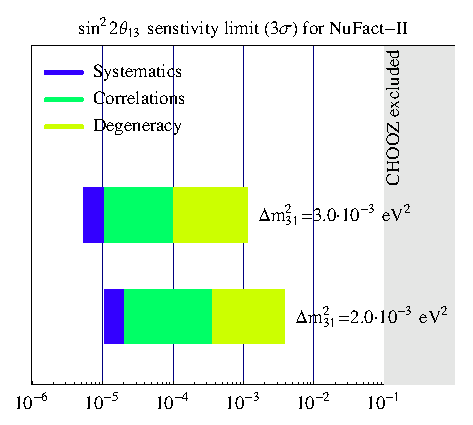
\includegraphics[width=6.5cm]{barsex}}
\end{center}
}

\section{Systematics}
\label{sec:systematics}
\index{Systematics}
\index{Systematics on/off}

Changing the systematics at running time can be useful to investigate
the impact factors affecting the measurement.
In \GLOBES , the systematics is defined rule-based, \ie, each rule
has its own systematics. In addition, \AEDL\ requires that it has to be
defined in each rule what ``Systematics on'' and ``Systematics off'' means.
Therefore, it is usually very simple to switch the systematics on and off:
\begin{function}
\GLBNS{glbSwitchSystematics}
{\tt int glbSwitchSystematics(int exp, int rule, int on\_off)}
switches the systematics in experiment {\tt exp} and rule {\tt rule}
on ({\tt on\_off} is \GLB{GLB\_ON}) or off ({\tt on\_off} is \GLB{GLB\_OFF}). For the experiment or
rule index, one can also use \GLB{GLB\_ALL}. 
\end{function}
In the example on page~\pageref{ex:barcharts}, the application of
{\tt glbSwitchSystematics} is demonstrated to show the impact of
systematics, correlations, and degeneracies.

\index{Error dimension}
The error dimension (for the definition, see \Sec~\ref{sec:rules}) can also be accessed directly with 
\begin{function}
\GLBNS{glbSetErrorDim}
{\tt int glbSetErrorDim(int exp, int rule, int on\_off, int value)}
sets the error dimension for systematics on ({\tt on\_off} is \GLB{GLB\_ON}) or off ({\tt on\_off} is \GLB{GLB\_OFF}) of experiment {\tt exp} and rule {\tt rule} to the value {\tt value}. The function returns
$-1$ if not successful.
\end{function}
\begin{function}
\GLBNS{glbGetErrorDim}
{\tt int glbGetErrorDim(int exp, int rule, int on\_off)}
returns the error dimension for systematics on ({\tt on\_off} is \GLB{GLB\_ON}) or off ({\tt on\_off} is \GLB{GLB\_OFF}) of experiment {\tt exp} and rule {\tt rule}.
\end{function}

\index{Signal errors}
\index{Background errors}
\index{Background centers}
Except from the general treatment of systematics, one can read out
and write the signal and background errors, as well as the background
centers. For the definitions of these quantities, see \Sec~\ref{sec:rules}.
\begin{function}
\GLBNS{glbSetSignalErrors}
{\tt int glbSetSignalErrors(int exp, int rule, double norm, double tilt)}
sets the signal errors of experiment {\tt exp} and rule {\tt rule}
to {\tt norm} (normalization error) and {\tt tilt} (tilt/calibration error).
\end{function}
\begin{function}
\GLBNS{glbGetSignalErrors}
{\tt int glbGetSignalErrors(int exp, int rule, double* norm, double* tilt)}
writes the signal errors of experiment {\tt exp} and rule {\tt rule}
to {\tt norm} (normalization error) and {\tt tilt} (tilt/calibration error).
\end{function}
\begin{function}
\GLBNS{glbSetBGErrors}
{\tt int glbSetBGErrors(int exp, int rule, double norm, double tilt)}
sets the background errors of experiment {\tt exp} and rule {\tt rule}
to {\tt norm} (normalization error) and {\tt tilt} (tilt/calibration error).
\end{function}
\begin{function}
\GLBNS{glbGetBGErrors}
{\tt int glbGetBGErrors(int exp, int rule, double* norm, double* tilt)}
writes the background errors of experiment {\tt exp} and rule {\tt rule}
to {\tt norm} (normalization error) and {\tt tilt} (tilt/calibration error).
\end{function}
\begin{function}
\GLBNS{glbSetBGCenters}
{\tt int glbSetBGCenters(int exp, int rule, double norm, double tilt)}
sets the background centers of experiment {\tt exp} and rule {\tt rule}
to {\tt norm} (normalization center) and {\tt tilt} (tilt/calibration center).
\end{function}
\begin{function}
\GLBNS{glbGetBGCenters}
{\tt int glbGetBGCenters(int exp, int rule, double* norm, double* tilt)}
writes the background centers of experiment {\tt exp} and rule {\tt rule}
to {\tt norm} (normalization center) and {\tt tilt} (tilt/calibration center).
\end{function}
As usual, all these functions return $-1$ if they were not successful.

\section{External parameters in \AEDL\ files}
\label{sec:aedlparams}
\index{External \AEDL\ parameters}

Using external parameters in \AEDL\ files is a very powerful feature
to change experiment parameters at running time which require that
the experiment be re-initialized. For example, one can change the
energy resolution function or the number of energy bins. However,
in some cases there might be complications, such that the number
of pre- or post-smearing efficiencies does not correspond to the number
of energy bins anymore. Therefore, this feature needs to be 
used with care.

In order to use external parameters in \AEDL\ files, one simply
introduces them. For example, an energy resolution function
\begin{quote}
{\tt
energy(\#EnergyResolution1)< \\
\hspace*{1cm} type = 1 \\
\hspace*{1cm} @sigma\_e = \{ myres ,0,0 \} \\
> \\
}
\end{quote}
might be defined in \AEDL , where the energy resolution is proportional
to {\tt myres} $\times$ energy. 

In order to use the user-defined variable, one has to assign it 
with {\tt glbDefineAEDLVariable} {\em before} the experiment is initialized with \GLB{glbInitExperiment}:
\begin{function}
\GLBNS{glbDefineAEDLVariable}
{\tt void glbDefineAEDLVariable(const char* name, double value)}
assigns the value {\tt value} to the \AEDL\ variable {\tt name}.
\end{function}
In our energy resolution example, one could now loop over the
energy resolution such as with
\begin{quote}
{\tt
int i; \\
for(i=5;i<20;i++) \\
\{ \\    
\hspace*{1cm} glbClearExperimentList(); \\
\hspace*{1cm} glbDefineAEDLVariable("myres",0.01*i); \\
\hspace*{1cm} glbInitExperiment(...); \\
\\
\hspace*{1cm} /* do something */ \\
\}
}
\end{quote}
Note that one does not have do re-initialize the oscillation
parameter vectors every time within the loop as long as the
number of experiments does not change.

In order to clear the external variable stack if one is
excessively using it, one can use
\begin{function}
\GLBNS{glbClearAEDLVariables}
{\tt void glbClearAEDLVariables()}
clears the \AEDL\ variable list.
\end{function}
This function is called automatically upon exit of the program.

\section{Algorithm parameters: Filter functions}
\index{Filter functions}

The oscillation frequency filters to filter fast oscillations
can also be accessed by the user interface. For details of
the filter functions, we refer to \Sec~\ref{sec:energy} of
the \AEDL\ manual.

In particular, there are a number of functions:
\begin{function}
\GLBNS{glbSetFilterState}
{\tt int glbSetFilterState(int on\_off)} sets the filter state to
on (\GLB{GLB\_ON}) or off (\GLB{GLB\_OFF}).
\end{function}
\begin{function}
\GLBNS{glbGetFilterState}
{\tt int glbGetFilterState()} returns the filter state.
\end{function}
\begin{function}
\GLBNS{glbSetFilterStateInExperiment}
{\tt int glbSetFilterStateInExperiment(int exp, int on\_off)} sets the filter state in experiment {\tt exp} to on (\GLB{GLB\_ON}) or off (\GLB{GLB\_OFF}).
\end{function}
\begin{function}
\GLBNS{glbGetFilterStateInExperiment}
{\tt int glbGetFilterStateInExperiment(int exp)} returns the filter state of experiment {\tt exp}.
\end{function}
Analogously, the filter value can be accessed:
\begin{function}
\GLBNS{glbSetFilter}
{\tt int glbSetFilter(double filter)} sets the filter to the
value {\tt filter}.
\end{function}
\begin{function}
\GLBNS{glbGetFilter}
{\tt double glbGetFilter()} returns the filter value.
\end{function}
\begin{function}
\GLBNS{glbSetFilterInExperiment}
{\tt int glbSetFilterInExperiment(int exp, double filter)} sets the filter  in experiment {\tt exp} to the value {\tt value}.
\end{function}
\begin{function}
\GLBNS{glbGetFilterInExperiment}
{\tt double glbGetFilterInExperiment(int exp)} returns the filter value of experiment {\tt exp}.
\end{function}
The return value of all {\tt Set-} functions is $-1$ if they were not successful.
